%=================================================================
% Neutral (venue-independent) LaTeX preamble for CLOP-DiT manuscript.
% Replaces the MDPI Definitions/mdpi class with a standard article class.
% MDPI-specific macros (\Title, \Author, \abstract{}, \keyword,
% \authorcontributions, \funding, etc.) are shimmed below so the body
% stays untouched.  Original MDPI source preserved at
%   clop_dit_genes.tex.mdpi_backup
%=================================================================

\documentclass[11pt,a4paper]{article}

% --- Core packages (MDPI class auto-loaded most of these) ---
\usepackage[utf8]{inputenc}
\usepackage[T1]{fontenc}
\usepackage[margin=1in]{geometry}
\usepackage{amsmath,amssymb,amsthm}
\usepackage{graphicx}
\usepackage{xcolor}
\usepackage{colortbl}
\usepackage{array}
\usepackage{booktabs}
\usepackage{multirow}
\usepackage{tabularx}
\usepackage{longtable}
% MDPI tabularx convention: C = centered X (centered version of auto-width column)
\newcolumntype{C}{>{\centering\arraybackslash}X}
\newcolumntype{L}{>{\raggedright\arraybackslash}X}
\newcolumntype{R}{>{\raggedleft\arraybackslash}X}
\usepackage{microtype}
\usepackage{titlesec}
\usepackage{etoolbox}
\usepackage{caption}
\usepackage{placeins}
\usepackage{float}
\usepackage{lineno}
\usepackage{changepage}
\usepackage{upgreek}
\usepackage{setspace}
\usepackage{enumitem}
\usepackage[numbers,square,sort&compress]{natbib}
\usepackage[colorlinks=true,linkcolor=black,citecolor=black,urlcolor=blue]{hyperref}
\usepackage{cleveref}
\usepackage{url}

% --- Spacing / layout: production-grade tight float placement ---
\raggedbottom
\setlength{\headheight}{20pt}
\setlength{\textfloatsep}{4pt plus 1.0pt minus 1.0pt}
\setlength{\floatsep}{4pt plus 1.0pt minus 1.0pt}
\setlength{\intextsep}{4pt plus 1.0pt minus 1.0pt}
\renewcommand{\topfraction}{0.97}
\renewcommand{\bottomfraction}{0.93}
\renewcommand{\textfraction}{0.03}
\renewcommand{\floatpagefraction}{0.90}
\setcounter{topnumber}{6}
\setcounter{bottomnumber}{4}
\setcounter{totalnumber}{12}
\setlength{\abovecaptionskip}{2pt}
\setlength{\belowcaptionskip}{1pt}
\setlength{\parskip}{3pt plus 1pt minus 0.5pt}
\AtBeginDocument{%
  \setlength{\abovedisplayskip}{6pt plus 2pt minus 2pt}%
  \setlength{\belowdisplayskip}{6pt plus 2pt minus 2pt}%
  \setlength{\abovedisplayshortskip}{3pt plus 1pt minus 1pt}%
  \setlength{\belowdisplayshortskip}{3pt plus 1pt minus 1pt}%
}
\titlespacing{\section}{0pt}{8pt}{2pt}
\titlespacing{\subsection}{0pt}{8pt}{2pt}
\titlespacing{\subsubsection}{0pt}{8pt}{2pt}
\titlespacing{\paragraph}{0pt}{6pt}{2pt}

% ================================================================
% MDPI-command shims: accept and render in a neutral style so the
% body (authored against the MDPI class) compiles unchanged.
% ================================================================

% ORCID rendering — MDPI class defined \orcidA as a small badge; here
% we just render the linked id plainly if the ORCID newcommand is set.
\newcommand{\orcidA}{}  % no-op (ORCID id is in \newcommand{\orcidauthorA})

% Title / author / abstract / keyword — MDPI uses commands with a
% single argument, not standard environments.  Store into locals and
% emit a standard \maketitle-style header at begin-document.
\makeatletter
\newcommand{\@mdpititle}{}
\newcommand{\@mdpiauthor}{}
\newcommand{\@mdpiaddress}{}
\newcommand{\@mdpicorres}{}
\newcommand{\@mdpiabstract}{}
\newcommand{\@mdpikeyword}{}
\providecommand{\Title}[1]{}\renewcommand{\Title}[1]{\renewcommand{\@mdpititle}{#1}}
\providecommand{\Author}[1]{}\renewcommand{\Author}[1]{\renewcommand{\@mdpiauthor}{#1}}
\providecommand{\AuthorNames}[1]{}\renewcommand{\AuthorNames}[1]{}
\providecommand{\address}[1]{}\renewcommand{\address}[1]{\renewcommand{\@mdpiaddress}{#1}}
\providecommand{\corres}[1]{}\renewcommand{\corres}[1]{\renewcommand{\@mdpicorres}{#1}}
\renewcommand{\abstract}[1]{\renewcommand{\@mdpiabstract}{#1}}
\providecommand{\keyword}[1]{}\renewcommand{\keyword}[1]{\renewcommand{\@mdpikeyword}{#1}}
\providecommand{\simplesumm}[1]{}\renewcommand{\simplesumm}[1]{}
\newcommand{\mdpiemitheader}{%
  \begin{center}
    {\LARGE\bfseries \@mdpititle \par}
    \vspace{0.6em}
    {\large \@mdpiauthor \par}
    \vspace{0.3em}
    {\small \@mdpiaddress \par}
    \vspace{0.2em}
    {\small \@mdpicorres \par}
  \end{center}
  \vspace{0.3em}
  % Render abstract manually: \abstract was renewed as a one-arg macro above,
  % so \begin{abstract} breaks. Emit an indented quoted paragraph instead.
  \ifx\@mdpiabstract\@empty\else
    \begingroup
      \leftskip=1.5em \rightskip=1.5em \small
      \noindent\textbf{Abstract:}\ \@mdpiabstract\par
    \endgroup
    \vspace{0.6em}
  \fi
  \ifx\@mdpikeyword\@empty\else
    \noindent\textbf{Keywords:}\ \@mdpikeyword\par\vspace{0.6em}
  \fi
}
\makeatother

% Matter-end macros (MDPI class provided these as section-emitters).
\newcommand{\abbreviations}[2]{\section*{#1}#2}
\newcommand{\authorcontributions}[1]{\section*{Author Contributions}#1}
\newcommand{\funding}[1]{\section*{Funding}#1}
\newcommand{\institutionalreview}[1]{\section*{Institutional Review Board Statement}#1}
\newcommand{\informedconsent}[1]{\section*{Informed Consent Statement}#1}
\newcommand{\dataavailability}[1]{\section*{Data Availability Statement}#1}
\newcommand{\acknowledgments}[1]{\section*{Acknowledgments}#1}
\newcommand{\conflictsofinterest}[1]{\section*{Conflicts of Interest}#1}
\newcommand{\reftitle}[1]{\section*{#1}}

% Additional MDPI-style shims
\newcommand{\useofartificialintelligence}[1]{\section*{Use of AI-Assisted Tools}#1}
\newcommand{\appendixtitles}[1]{}  % MDPI toggle for appendix title style — no-op
\newcommand{\appendixstart}{\appendix}  % MDPI appendix-start marker
\newlength{\extralength}
\setlength{\extralength}{0pt}  % MDPI margin extension — zero under article
\newcommand{\PublishersNote}[1]{}  % MDPI publisher's note — hidden

% MDPI no-op internals (page/issue/doi/date metadata — not needed here).
\newcommand{\firstpage}[1]{}
\newcommand{\pubvolume}[1]{}
\newcommand{\issuenum}[1]{}
\newcommand{\articlenumber}[1]{}
\newcommand{\pubyear}[1]{}
\newcommand{\copyrightyear}[1]{}
\newcommand{\datereceived}[1]{}
\newcommand{\daterevised}[1]{}
\newcommand{\dateaccepted}[1]{}
\newcommand{\datepublished}[1]{}
\newcommand{\doinum}[1]{}

% Re-emit \maketitle-equivalent right after begin-document so
% \Title / \Author / \abstract / \keyword appearing in the preamble
% actually render.  We shim this via \AtBeginDocument.
\AtBeginDocument{\mdpiemitheader}

%=================================================================
% Title / author / affiliation / corresponding author / abstract /
% keywords — restored after the MDPI → neutral-template swap.  The
% neutral preamble above stores these strings and emits them via
% \mdpiemitheader at \begin{document}.
%=================================================================

\Title{CLOP-DiT: Structured-Metadata-Conditioned Single-Cell Latent Generation via Contrastive Language-Omics Pretraining and Diffusion Transformers}

\newcommand{\orcidauthorA}{0009-0001-8329-0108}

\Author{Zeyu Fu$^{1,\dagger,*}$, Yiyao Liu$^{1,\dagger}$, Junping Wang$^{1,*}$, Song Wang$^{1,*}$}
\AuthorNames{Zeyu Fu, Yiyao Liu, Junping Wang, Song Wang}

\address{%
$^{1}$~State Key Laboratory of Trauma and Chemical Poisoning, Institute of Combined Injury, Chongqing Engineering Research Center for Nanomedicine, College of Preventive Medicine, Army Medical University, Chongqing 400038, China\\
$^{\dagger}$~These authors contributed equally\\
$^{*}$~Corresponding authors}

\corres{Correspondence: \href{mailto:fuzeyu09@gmail.com}{fuzeyu09@gmail.com} (Zeyu Fu, primary corresponding author)}

% Abstract — updated per Reviewer 2 Comment 2.1: added a background
% sentence on the current field of single-cell generation and an
% explicit challenge sentence before moving into method and results.
\abstract{Single-cell RNA sequencing has transformed cellular heterogeneity analysis, but most single-cell generative models are conditioned on narrow categorical labels such as cell type, batch, or perturbation rather than structured biological descriptions. This limits controlled simulation and hypothesis-guided exploration, especially when biologically meaningful within-type heterogeneity must be preserved. We present CLOP-DiT, a three-stage framework for structured-metadata-conditioned single-cell latent generation. CLOP first aligns frozen BiomedBERT text embeddings and frozen scGPT cell embeddings in a shared 512-dimensional space. A conditional 1-D Diffusion Transformer then performs flow matching in this latent space under a fixed five-field prompt template covering cell type, tissue, organism, marker genes, and disease context. Finally, a frozen scGPT decoder maps generated latents back to gene expression for inspection. Across 69 deduplicated cell types from 80 GEO datasets (220{,}304 cells), a high-fidelity regime (CFG\,=\,2.0) achieves 36.9\% KNN accuracy, approximately $25\times$ random chance, and 81.0\% steering. A high-diversity regime (CFG\,=\,1.0) reaches a diversity ratio of 0.93 while retaining 80.7\% steering. Conditioning-field ablation and swap-label tests identify marker genes as the strongest steering signal, with steering falling from 99.8\% under the full prompt to 62.4\% with metadata alone. We also report current limits: cross-dataset variance correlation remains near zero, discriminator AUC is 0.656, and rare-cell augmentation remains negative. CLOP-DiT therefore supports controllable structured-metadata generation while highlighting the remaining challenge of preserving within-type heterogeneity and downstream biological realism.}

\keyword{single-cell RNA-seq; generative model; diffusion transformer; contrastive learning; structured-metadata conditioning; flow matching; latent generation; foundation model}

%=================================================================

\begin{document}

%%%%%%%%%%%%%%%%%%%%%%%%%%%%%%%%%%%%%%%%%%
\section{Introduction}

Single-cell RNA sequencing (scRNA-seq) has transformed the study of cellular heterogeneity by enabling transcriptome-scale profiling at single-cell resolution~\cite{ref-scrnaseq-review,ref-10x}. Yet the inverse problem---generating new cell states from structured biological descriptors---remains difficult. A useful model would need not only to synthesize plausible transcriptomes, but also to preserve biologically meaningful condition-specific structure across cell identity, tissue context, organism, marker genes, and disease state.

Most existing single-cell generative models condition on categorical labels, perturbation labels, or batch covariates rather than on richer multi-field biological descriptions. Variational autoencoders such as scVI~\cite{ref-scvi,ref-scvi-tools} and scGen~\cite{ref-scgen}, geometry-aware generative models~\cite{ref-scdiff}, and recent foundation-model approaches such as Geneformer, scBERT, scFoundation, CellPLM, and UCE~\cite{ref-geneformer,ref-scbert,ref-scfoundation,ref-cellplm,ref-uce} have broadened the modeling landscape, but they do not jointly learn a structured text--cell alignment space and a diffusion-style conditional generator. Language-mediated methods such as Cell2Sentence~\cite{ref-cell2sentence} and GenePT~\cite{ref-genept} extend the role of text in single-cell analysis, yet they address different tasks and do not synthesize new single-cell expression profiles from aligned biological descriptions.

The closest conceptual comparator is CellWhisperer~\cite{ref-cellwhisperer}, which likewise connects natural language and single-cell transcriptomics through contrastive alignment. CellWhisperer, however, is fundamentally \emph{discriminative}: it retrieves and annotates existing cells from a reference atlas. CLOP-DiT targets the complementary \emph{generative} setting. Given a structured biological description, it synthesizes new cell states rather than retrieving existing ones. That distinction matters for applications such as rare-cell augmentation, in silico condition simulation, and controlled hypothesis generation. Table~\ref{tab:method-comparison} summarizes the methodological differences.

\begin{table}[!htbp]
\caption{Comparison of CLOP-DiT with related methods for conditional single-cell generation and annotation. ``Cond.\ modality'' indicates the conditioning input type; ``Gen.\ paradigm'' indicates the generation approach.\label{tab:method-comparison}}
\centering
\small
\begin{tabular}{lccc}
\toprule
\textbf{Method} & \textbf{Cond.\ Modality} & \textbf{Gen.\ Paradigm} & \textbf{Output} \\
\midrule
scVI~\cite{ref-scvi}           & Categorical (batch/type) & cVAE               & Expression \\
scGen~\cite{ref-scgen}         & Categorical (perturbation) & VAE + shift       & Expression \\
Geneformer~\cite{ref-geneformer} & Rank-value tokens & Masked LM           & Cell embeddings \\
Cell2Sentence~\cite{ref-cell2sentence} & Gene-rank text   & LLM decoding        & Gene-rank text \\
GenePT~\cite{ref-genept}       & Gene text embeddings     & None (annotation)   & Annotations \\
CellWhisperer~\cite{ref-cellwhisperer} & Free-form text           & None (retrieval)    & Cell annotations \\
\textbf{CLOP-DiT (ours)}       & \textbf{Structured 5-field text} & \textbf{DiT + flow matching} & \textbf{Gene expression} \\
\bottomrule
\end{tabular}
\end{table}

Recent progress in contrastive multimodal learning and continuous generative modeling provides the ingredients for such a system. CLIP/SigLIP-style objectives can align heterogeneous modalities in a shared embedding space~\cite{ref-clip,ref-siglip}, whereas Diffusion Transformers and flow matching support scalable conditional generation in continuous latent spaces~\cite{ref-dit,ref-flow-matching,ref-albergo-flow,ref-rectified-flow}. CLOP-DiT combines these ideas in a domain-specific way: it first constructs a well-separated text--cell conditioning space and then learns a conditional sampler in scGPT latent space.

CLOP-DiT is organized as a three-stage pipeline. CLOP aligns structured metadata with scGPT cell embeddings; DiT samples new scGPT-compatible latents from that aligned condition; and a frozen scGPT decoder maps those latents back to gene expression for downstream biological inspection. The input prompt is a fixed five-field template---cell type, tissue, organism, marker genes, and disease context---so the task is best understood as structured-metadata conditioning rather than free-form language understanding.

The main contributions are fourfold. First, we introduce a prototype-aware contrastive aligner that combines whitened encoder embeddings with shared 512-dimensional projection heads to produce a well-separated condition space. Second, we train a 1D Diffusion Transformer to generate type-specific cell embeddings under structured text conditioning. Third, we evaluate the model on 69 deduplicated cell types from 80 GEO studies using complementary latent, diversity, and downstream biological metrics. Fourth, we report both strengths and limitations: the model achieves clear above-chance type specificity and controllable fidelity--diversity trade-offs, but variance preservation, covariance preservation, and rare-cell augmentation remain incomplete.

Across two primary operating regimes, CLOP-DiT reaches 36.9\% KNN accuracy and 81.0\% steering in a high-fidelity setting, whereas a high-diversity setting attains a diversity ratio of 0.93 at 80.7\% steering. We therefore position CLOP-DiT as a structured-metadata-conditioned single-cell generation framework that is already informative, but not yet a drop-in simulator for downstream biological inference. Concretely, the \emph{primary target} of this work is controllable, biologically faithful single-cell latent generation from structured metadata, evaluated jointly on type specificity, prompt-driven steering controllability, and within-type heterogeneity preservation; each remaining gap in these three axes is diagnosed explicitly in the Results and Discussion rather than masked by a single composite headline number.

%%%%%%%%%%%%%%%%%%%%%%%%%%%%%%%%%%%%%%%%%%
\section{Materials and Methods}

Figure~\ref{fig:architecture} summarizes the full workflow. For clarity, the Materials and Methods are organized in three parts: (1) dataset curation, caption construction, and embedding preprocessing (\ref{sec:dataset}); (2) model architecture and training, covering CLOP alignment (\ref{sec:clop}), DiT generation (\ref{sec:dit}), and scGPT decoding (\ref{sec:decoding}); and (3) evaluation metrics, operating points, and statistical reporting (\ref{sec:evaluation}). This ordering follows the actual data flow from GEO-derived cells and structured captions to latent generation and downstream biological validation.

\begin{figure}[!htbp]
\centering
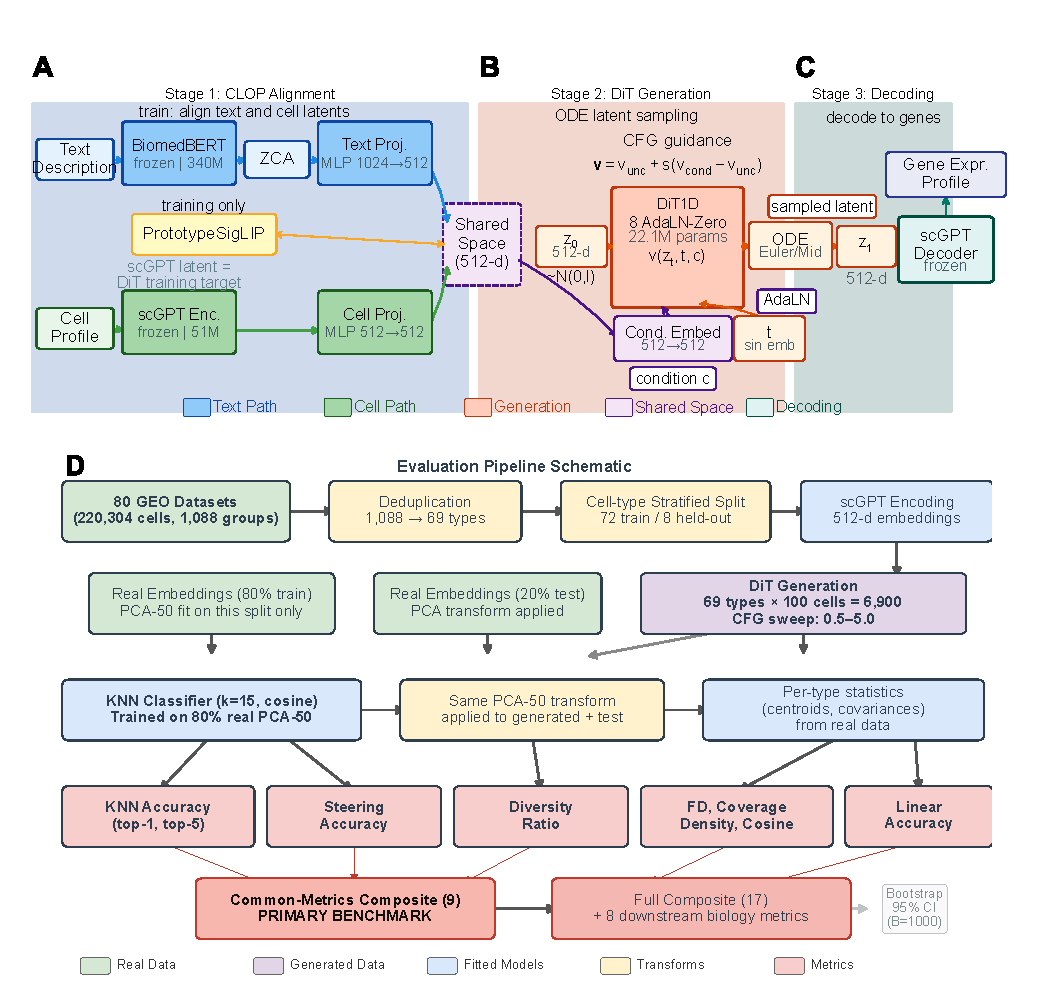
\includegraphics[width=\textwidth]{Figure_01_pipeline_overview.pdf}
\caption{\textbf{CLOP-DiT pipeline overview and evaluation framework.} \textbf{(Top)} \textbf{A--C}: Stage~1 (CLOP) aligns structured text descriptions and scGPT cell embeddings in a shared 512-dimensional space after BiomedBERT whitening and projection; Stage~2 (DiT) performs conditional flow matching in scGPT latent space and samples a target latent from Gaussian noise with classifier-free guidance; Stage~3 (Decoding) maps the sampled latent back to gene expression through the frozen scGPT decoder. \textbf{(Bottom)} \textbf{D}: evaluation pipeline schematic from raw datasets through deduplication, stratified splitting, scGPT encoding, PCA fitting on the real-training split, KNN training, and metric computation. The common-metrics-only composite (9 shared distributional metrics) is the primary benchmark; bootstrap confidence intervals ($B{=}1{,}000$) are computed by resampling the 69 evaluation types.\label{fig:architecture}\label{fig:eval-pipeline}}
\end{figure}

\subsection{Datasets and preprocessing}\label{sec:dataset}

We curated 80 scRNA-seq datasets from the Gene Expression Omnibus (GEO), spanning cancer and developmental biology and totaling 220,304 cells after quality control and highly variable gene selection~\cite{ref-seurat,ref-hvg}. For each dataset, 2,000 highly variable genes were retained. Each cell was then encoded as a 512-dimensional embedding by a pre-trained scGPT model. Cell-type annotations were organized into 1,088 unique text groups, each represented by a structured caption rather than free-form prose. These captions combine cell type, marker genes, tissue of origin, organism, and disease context using the following template:
\begin{quote}\small\ttfamily
\{cell type\}, tissue: \{tissue\}, organism: \{organism\},\\
markers: \{top 5 DE marker genes\}, context: \{disease/condition\}
\end{quote}
\noindent Marker genes were identified by one-vs.-rest Wilcoxon rank-sum testing on the training split~\cite{ref-wilcoxon}. To check that these markers were not merely circular artifacts of the training corpus, we compared them against PanglaoDB~\cite{ref-panglao} and CellMarker~2.0~\cite{ref-cellmarker}. The resulting Jaccard overlap (0.39--0.45, well above the ${\sim}$0.01 expected for random gene sets of this size) indicates substantial agreement with external biological knowledge (see Discussion). The exact caption template and marker-gene sources are provided in the project repository~\cite{ref-clop-dit}.

Before CLOP training, both BiomedBERT text embeddings and scGPT cell embeddings were preprocessed upstream by mean-centering, ZCA whitening, and $L_2$ normalization using statistics estimated from the training data. Text preprocessing was fit on unique captions to avoid overweighting duplicated descriptions, whereas cell preprocessing was fit on a 50,000-cell training subsample for efficiency and then applied to the full corpus. As a result, the contrastive aligner operates on preprocessed encoder outputs rather than learning whitening inside the network.

The corpus was split into 72 training datasets (199,670 cells) and 8 held-out validation datasets (20,634 cells). Validation was defined at the study level rather than the cell level so that no samples overlap between training and validation. The held-out studies were chosen by stratified selection across the major tissue and cancer categories represented in the corpus (lung, gastric, skin, liver, blood). The full list of 80 GEO accession identifiers is provided in Table~\ref{tab:s1_datasets} (Appendix~\ref{app:suppl-tables}), and the validation studies are listed in Table~\ref{tab:s2_validation}. Within the training studies, a cell-type-stratified split reserves approximately 10\% of cells per type for training-time validation, ensuring that all 69 deduplicated evaluation types are represented in both partitions. This design therefore tests interpolation within the observed training distribution rather than stringent out-of-distribution generalization.

The relationship between the 1,088 text groups and the 69 evaluated cell types is as follows. The 1,088 text groups correspond to sub-cluster-level descriptions: each Leiden~\cite{ref-leiden} cluster within each dataset receives its own caption. Many sub-clusters nevertheless map to the same canonical cell type (for example, ``CD8+ T cells'' appearing in distinct tissues or studies). For evaluation, these text groups are consolidated by core identity through a deduplication pipeline that (a)~removes ambiguous or uncharacterized sub-clusters and (b)~merges cross-dataset sub-clusters into canonical types, yielding 69 evaluable cell types. The resulting deduplicated evaluation set contains 167,245 cells and is the basis for all headline generation metrics, bootstrap confidence intervals, and benchmark comparisons. KNN accuracy is therefore reported over a consistent 69-type problem (random chance = $1/69 \approx 1.45\%$).

The 80 datasets include both \textit{Homo sapiens} (59 datasets) and \textit{Mus musculus} (21 datasets, including Tabula Muris~\cite{ref-tabula-muris}) and are dominated by tumor-microenvironment and developmental contexts. All claims in this study should therefore be interpreted within that scope; generalization to other organisms, non-cancer tissues, or perturbation-heavy settings has not been tested. Training and evaluation were implemented in Python~3.10 using PyTorch~2.1 (CUDA~12.0), scGPT~v0.2.1, and Hugging Face Transformers~4.36 for BiomedBERT; the complete environment specification is available in the project repository~\cite{ref-clop-dit}.

\paragraph{Hardware and compute budget.}
All training and evaluation were conducted on a single NVIDIA GeForce RTX~5090 Laptop GPU (24\,GB VRAM) using PyTorch~2.1 with CUDA~12.0 and automatic mixed precision (AMP/FP16). The total compute budget remains modest ($<$2 GPU-hours in aggregate, $<$24\,GB VRAM peak), so reproduction should be feasible on any Ampere-or-later GPU with at least 16\,GB VRAM. CLOP alignment training completes in minutes, DiT training in roughly an hour-scale run, and end-to-end figure regeneration from saved latent representations in under 30~minutes. No multi-GPU or distributed training was used. Inference for 69 cell types (approximately 6,900 generated cells) takes about 2~minutes with 10-step Euler integration.

\subsection{CLOP: Contrastive Language--Omics Pretraining}\label{sec:clop}

CLOP aligns structured metadata descriptions and cell profiles in a shared 512-dimensional embedding space, producing the condition representation used by the DiT. A frozen BiomedBERT-large encoder maps captions to 1024-dimensional embeddings, and a frozen scGPT encoder maps cells to 512-dimensional embeddings. The production aligner uses dual three-layer MLP projectors (text: $1024 \to 1024 \to 1024 \to 512$; cell: $512 \to 512 \to 512 \to 512$) with LayerNorm, GELU activation~\cite{ref-gelu}, and dropout~\cite{ref-dropout} (0.2), followed by $L_2$ normalization onto the unit hypersphere. In the final configuration, duplicate captions within a mini-batch are masked so that cells sharing the same caption are not treated as false negatives.

Because many cells share the same caption, the production objective is not a pure instance-level cross-entropy loss. Instead, CLOP uses a PrototypeSigLIP loss that aligns one representative text projection per caption group to the centroid of the corresponding cell projections within the batch. Let $S_g$ denote the set of cells in group $g$, $\mathbf{c}_i$ the projected cell embedding of cell $i$, and
\begin{linenomath}
\begin{equation}
\mathbf{p}_g = \mathrm{norm}\!\left(\frac{1}{|S_g|}\sum_{i \in S_g} \mathbf{c}_i\right)
\end{equation}
\end{linenomath}
the normalized prototype for that group. With representative text projection $\mathbf{t}_g$, learned bias $b$, and fixed logit scale $\tau$, the prototype-alignment term is

\begin{linenomath}
\begin{equation}
\ell_{gh} = \tau\,\mathbf{t}_g^\top \mathbf{p}_h + b, \qquad
\mathcal{L}_\text{align} = -\frac{1}{G^2}\sum_{g=1}^{G}\sum_{h=1}^{G}\log\sigma\!\left(y_{gh}\,\ell_{gh}\right),
\label{eq:clop}
\end{equation}
\end{linenomath}

where $y_{gh}=1$ when $g=h$ and $y_{gh}=-1$ otherwise, $G$ is the number of caption groups in the batch, and $\sigma(\cdot)$ is the sigmoid function. A cohesion penalty then pulls individual cell projections toward their group prototype:

\begin{linenomath}
\begin{equation}
\mathcal{L}_\text{CLOP} = \mathcal{L}_\text{align} + \lambda_\text{coh}\,\frac{1}{B}\sum_{i=1}^{B}\left(1 - \mathbf{c}_i^\top \mathrm{sg}(\mathbf{p}_{g(i)})\right),
\end{equation}
\end{linenomath}

with $\lambda_\text{coh}=0.15$, batch size $B$, and $\mathrm{sg}(\cdot)$ denoting stop-gradient. In the production configuration, the SigLIP logit scale is fixed at $\tau = 14.0$ rather than learned. The aligner has 3.02M trainable parameters and is optimized with AdamW~\cite{ref-adamw} (lr~$= 5 \times 10^{-4}$, weight decay 0.06, cosine schedule~\cite{ref-cosine-schedule} with 5-epoch warmup) over a 100-epoch training run.

The key output of CLOP is the projected condition space. Raw scGPT cell-type centroids have a mean pairwise cosine similarity of 0.994 (that is, cell types differ by only 0.6\% on average), whereas CLOP-projected conditions reduce this mean to 0.222, increasing inter-group separation by approximately $130\times$. That improvement is what makes conditional generation in the subsequent DiT stage feasible.

\subsection{DiT: Conditional Flow Matching with Diffusion Transformer}\label{sec:dit}

The Diffusion Transformer (DiT1D) reshapes each 512-dimensional cell embedding into 16 pseudo-tokens of dimension 32. The backbone comprises 8 AdaLN-Zero transformer blocks with 8-head self-attention and an MLP expansion ratio of 4.0, corresponding to feed-forward sublayers of size $512 \to 2048 \to 512$. Timestep information and CLOP condition vectors are each projected to 512 dimensions and combined by element-wise summation, so every block is modulated by a shared conditioning signal rather than by concatenated inputs. The model has 22.10M trainable parameters (Table~\ref{tab:architecture}).

The base training objective is the standard flow-matching loss~\cite{ref-flow-matching,ref-ot-cfm}:

\begin{linenomath}
\begin{equation}
\mathcal{L}_\text{FM} = \| v_\theta(z_t, t, c) - (z_1 - z_0) \|_2^2,
\label{eq:fm}
\end{equation}
\end{linenomath}

where $z_0 \sim \mathcal{N}(0, I)$, $z_1$ is the real cell embedding, $z_t = (1-t)z_0 + tz_1$, and $t$ is drawn from a logit-normal distribution ($\mu{=}0, \sigma{=}1$), which concentrates training on intermediate timesteps where the velocity field is most complex~\cite{ref-sd3}. During training, classifier-free guidance (CFG)~\cite{ref-cfg} is implemented by dropping the condition with 15\% probability and replacing it with a \emph{learned} null condition token. At inference,

\begin{linenomath}
\begin{equation}
v_\text{guided} = v_\text{uncond} + s \cdot (v_\text{cond} - v_\text{uncond}),
\label{eq:cfg}
\end{equation}
\end{linenomath}

where $s$ is the guidance scale.

To reduce mean-collapse, the production DiT adds two group-aware regularizers on the reconstructed clean latent $\hat{z}_1 = z_t + (1-t)\,v_\theta(z_t,t,c)$: a per-group variance-matching term and a sliced covariance-matching term based on random one-dimensional projections. The full objective is therefore

\begin{linenomath}
\begin{equation}
\mathcal{L}_\text{DiT} = \mathcal{L}_\text{FM} + \lambda_\text{var}\,\mathcal{L}_\text{var} + \lambda_\text{cov}\,\mathcal{L}_\text{cov},
\label{eq:var-loss}
\end{equation}
\end{linenomath}

with $\lambda_\text{var}=0.10$ and $\lambda_\text{cov}=0.05$. Here, $\mathcal{L}_\text{var}$ matches per-dimension variance within each caption group, and $\mathcal{L}_\text{cov}$ matches the variance of random projected views of real and reconstructed clean latents, providing a sliced approximation to covariance preservation. DiT is optimized with AdamW for a 300-epoch training run using EMA~\cite{ref-ema} (decay = 0.9999), cosine learning-rate decay with 5-epoch warmup, AMP, and gradient clipping at 1.0.

\subsection{Decoding via scGPT}\label{sec:decoding}

Generated latent vectors $z_1 \in \mathbb{R}^{512}$ are mapped back to gene expression using the frozen scGPT decoder. This stage is useful for downstream biological inspection, but it also imposes an important limitation: the decoder is many-to-one, so distinct latents near the training manifold can decode to similar expression profiles. We therefore treat latent-space metrics---KNN accuracy, steering, diversity ratio, and centroid cosine---as the primary indicators of generative quality, whereas expression-space analyses are interpreted as compatibility checks on the full pipeline rather than as direct measures of latent fidelity. Relaxing this bottleneck will require either decoder fine-tuning or a lightweight trainable adapter.

\subsection{Evaluation Framework}\label{sec:evaluation}

We evaluate CLOP-DiT along six axes using in-distribution conditions (the actual CLOP-projected text embeddings from training data):

\begin{enumerate}
\item \textbf{KNN classification accuracy}: For each generated cell, a $k$-nearest-neighbor classifier ($k{=}15$, cosine metric, PCA-50 features) trained on 80\% of real data predicts its cell type. PCA is fitted on the real training split only and applied identically to generated embeddings; the same PCA transform is used across all method comparisons. Random chance is $1/69 \approx 1.45\%$. Because real cell-type centroids in scGPT space have pairwise cosine similarity of 0.994, small embedding perturbations can substantially affect KNN accuracy; the biological meaning of absolute KNN values therefore warrants caution.
\item \textbf{Steering accuracy}: For random cell-type pairs $(A, B)$, we generate cells conditioned on $A$ and test whether the generated centroid is closer to the real cluster $A$ than $B$ in centered space. Random chance is 50\%. \textbf{Note:} At intermediate-to-high CFG values (e.g., CFG$\,\geq\,$1.5) with multi-step solvers, steering accuracy can saturate at 1.0 with bootstrap CI [1.0, 1.0], indicating a ceiling effect; this metric loses discriminative power once guidance is sufficient.
\item \textbf{Diversity ratio}: Ratio of generated within-group variance to real within-group variance. Ideal is 1.0; values $<$1 indicate mode sharpening; values $>$1 indicate excess noise.
\item \textbf{Coverage and density}: Coverage measures the fraction of real samples that have at least one generated neighbor within the real data's KNN radius ($k{=}5$); it quantifies mode coverage. Density measures the average number of generated samples falling within each real sample's KNN radius, normalised by $k$; it quantifies precision. Both are computed in PCA-50 embedding space.
\item \textbf{Centroid cosine similarity}: The cosine similarity between the real and generated cell-type centroids, computed in the 512-dimensional scGPT embedding space (uncentered; $\text{cos}(\boldsymbol{\mu}_\text{real}, \boldsymbol{\mu}_\text{gen})$). Reported per-type and averaged across 69 types.
\item \textbf{Downstream biological concordance}: Clustering alignment (ARI~\cite{ref-ari}, NMI~\cite{ref-nmi}), classifier transfer, and differential expression concordance between real and generated data.
\end{enumerate}

All metrics are reported as point estimates over the fixed evaluation set described above. Two configurations are designated as \emph{primary operating points}: CFG\,=\,2.0 with 10-step Euler integration (high-fidelity regime) and CFG\,=\,1.0 with 10-step Midpoint integration (high-diversity regime). All other CFG and solver combinations in Appendix~\ref{app:suppl-tables} represent sensitivity analysis; no multiple-comparison correction was applied to these exploratory comparisons. Bootstrap 95\% confidence intervals for the composite benchmark scores are shown in Figure~\ref{fig:benchmark}I; variability across single-measurement metrics (KNN, steering, diversity ratio) is characterized by the CFG sweep (Appendix~\ref{app:suppl-tables}, Table~\ref{tab:cfg-sweep}).

\textbf{Caveat on Fr\'{e}chet Distance (FD).} FD~\cite{ref-fid} compares distributional moments (mean and covariance) between real and generated samples. While widely used for unconditional evaluation, FD can be misleading for \emph{conditional} generation: a model that reproduces the global marginal distribution but ignores conditioning achieves a low FD without having learned the target conditional. FD is therefore reported as a secondary metric throughout; the primary metrics (KNN accuracy, steering, diversity ratio) are specifically designed for conditional evaluation.

The biological evidence is organized by figure family: Figures~\ref{fig:markers}--\ref{fig:expr-analysis} establish marker-level and gene-level fidelity; Figures~\ref{fig:diversity} and~\ref{fig:expr-diversity} provide robustness readouts for guidance and diversity; Figure~\ref{fig:baselines} reports benchmarking; Figure~\ref{fig:downstream-pq} tests downstream biology. The evaluation pipeline is shown in the bottom panel of Figure~\ref{fig:eval-pipeline}.

\textbf{Metrics glossary.} The reader may consult the following one-line definitions for every metric reported in the Results and Discussion, in case a term is encountered outside its first-introduction paragraph. \emph{KNN top-1/top-5 accuracy}: fraction of generated cells whose top-1/top-5 KNN (cosine, $k{=}15$, PCA-50) predictions match the prompted cell type (random chance $\approx 1.45\%$). \emph{Steering accuracy}: fraction of $(A,B)$ pairs where the $A$-conditioned centroid is closer to real $A$ than to real $B$ (random chance $50\%$). \emph{Diversity Ratio (DivR)}: generated/real within-group variance; ideal $= 1$. \emph{Fr\'echet distance (FD)}: Gaussian distance between real and generated mean + covariance in the evaluation latent space; reported as a secondary distributional diagnostic only. \emph{Coverage, Density}: fraction of real samples with a generated neighbour within the real-KNN radius (coverage) and mean count of generated samples per real KNN ball normalised by $k$ (density), both on PCA-50. \emph{Centroid cosine}: cosine similarity between real and generated per-type centroids in the 512-d scGPT space. \emph{Linear classifier accuracy}: top-1 accuracy of a linear probe trained on PCA-50 real features and evaluated on generated cells. \emph{$r_\text{var}$}: Pearson correlation between per-gene variance of real and generated cells; pooled $r_\text{var}$ is computed across all types (\textit{first-order}), within-type $r_\text{var}$ is computed per cell type then summarised (\textit{second-order}). \emph{Mantel $r$}: Pearson correlation between per-type gene--gene correlation matrices of real vs.\ generated cells, evaluated on the top-50 HVG submatrix. \emph{SWD}: Sliced Wasserstein distance between per-type generated and real latent sets, averaged over random projections. \emph{Discriminator AUC}: area under the ROC curve of a logistic-regression real/generated discriminator trained on PCA-50 features; AUC $= 0.5$ denotes indistinguishability, AUC $= 1.0$ denotes perfect separation. \emph{Cluster purity}: fraction of dominant cell-type labels within each Leiden cluster of the real+generated mixture, evaluated alongside ARI and NMI in the downstream concordance pipeline.

Having established the methodology and evaluation framework, we now present the empirical results.

\subsection{Statistical Analysis}\label{sec:stats}

\textbf{Primary endpoints.} Two operating points were pre-specified as primary comparisons: CFG\,=\,2.0 with 10-step Euler integration (high-fidelity regime, selected because KNN accuracy plateaus at CFG 2.0--3.0 in Table~\ref{tab:cfg-sweep}; the lower end was chosen to minimize diversity loss) and CFG\,=\,1.0 with 10-step Midpoint integration (high-diversity regime, selected to match DivR\,$\approx$\,1.0). The primary metrics are KNN top-1 classification accuracy (69-class, $k{=}15$, cosine metric on PCA-50 features) and steering accuracy (pairwise directional test, 1000 random pairs).

\textbf{Exploratory analyses.} All other CFG/solver/step combinations reported in Tables~\ref{tab:cfg-sweep} and~\ref{tab:s3_cfg_sweep} (Appendix~\ref{app:suppl-tables}) constitute exploratory sensitivity analyses. No correction for multiple comparisons (e.g., Bonferroni, Holm) was applied to these comparisons. Rankings and performance claims refer only to the two primary operating points unless explicitly stated otherwise.

\textbf{Uncertainty quantification.} Bootstrap 95\% confidence intervals (percentile method, $B{=}1000$ resamples, seed 42) are reported for all headline metrics where per-unit (per-cell or per-type) data are available (see Results). These CIs capture evaluation sampling variability but not training-run variance, as all results derive from a single training run (seed 42). Formal superiority tests (e.g., permutation tests) were not conducted; all comparisons are descriptive.

\textbf{Multi-seed replication.} To characterize inter-run variance, we trained three independent CLOP + DiT pipeline replicas (seeds 42, 123, 456) with identical hyperparameters and report mean $\pm$ standard deviation for all core metrics in Table~\ref{tab:multi-seed} (see Section~\ref{sec:multi-seed-results}).

\textbf{Limitations of the statistical design.} (1)~No formal pre-registration: operating points were selected based on interpretable criteria post-hoc rather than by pre-registered protocol; this study is therefore exploratory rather than confirmatory. (2)~No multiple-comparison correction for the exploratory CFG sweep.

\subsection{Composite Score Formulation}\label{sec:composite}

The composite benchmark score aggregates all active metrics into a single ranking index. For each metric~$m$ with direction $d_m \in \{\text{lower}, \text{higher}\}$, let $v_{m,j}$ denote the raw value for method~$j$. We compute a min--max normalised score:
\begin{linenomath}
\begin{equation}
  s_{m,j} =
  \begin{cases}
    1 - \dfrac{v_{m,j} - \min_k v_{m,k}}{\max_k v_{m,k} - \min_k v_{m,k}} & \text{if } d_m = \text{lower},\\[6pt]
    \dfrac{v_{m,j} - \min_k v_{m,k}}{\max_k v_{m,k} - \min_k v_{m,k}} & \text{if } d_m = \text{higher},
  \end{cases}
  \label{eq:norm}
\end{equation}
\end{linenomath}
where $k$ ranges over all methods that report a non-null value for~$m$; methods lacking metric~$m$ receive $s_{m,j} = 0$. The composite score is the unweighted arithmetic mean over all~$M$ active metrics:
\begin{linenomath}
\begin{equation}
  C_j = \frac{1}{M}\sum_{m=1}^{M} s_{m,j}.
  \label{eq:composite}
\end{equation}
\end{linenomath}
Because not all methods support downstream biology (Section~\ref{sec:evaluation}, axis~6), they receive $s = 0$ on those metrics, which inflates the score of methods that do. In the current benchmark, 8 of 17 active metrics are reported only by CLOP-DiT; the remaining 9 distributional metrics are shared by all methods. \textbf{To enable fair like-for-like comparison, the common-metrics-only composite ($C_j^{\text{common}}$, restricted to the 9 shared distributional metrics) serves as the primary benchmark figure.} The full composite ($C_j$ over all $M = 17$ metrics) is reported as a supplementary capability ranking but should not be used for method comparison, as the 8 exclusive metrics structurally bias it in favor of CLOP-DiT. Table~\ref{tab:core-results} and the per-metric panels in Figure~\ref{fig:benchmark} report individual metrics for transparent comparison. Bootstrap 95\% confidence intervals (percentile method, $B{=}1{,}000$) for all headline generation metrics are provided in Table~\ref{tab:s5_bootstrap_ci} (Appendix~\ref{app:suppl-tables}).

%%%%%%%%%%%%%%%%%%%%%%%%%%%%%%%%%%%%%%%%%%
\FloatBarrier
\section{Results}\label{sec:results}

We report in-distribution results along the six evaluation axes defined in the Methods, organized by evidence type:
training dynamics and embedding space (Figure~\ref{fig:training});
core generation quality metrics and per-type analysis (Figure~\ref{fig:metrics});
gene-level fidelity (Figures~\ref{fig:markers}--\ref{fig:expr-analysis});
conditioning robustness and diversity trade-offs (Figures~\ref{fig:cond-umap},~\ref{fig:diversity}, and~\ref{fig:expr-diversity});
baseline comparisons and benchmarking (Figure~\ref{fig:baselines});
and downstream biological validation (Figure~\ref{fig:downstream-pq}).
This structure allows readers to assess evidence quality at multiple resolutions, from training convergence through partial downstream biological utility.

\subsection{Training Dynamics and Embedding Space}

Figure~\ref{fig:training} summarizes convergence across the two training stages. CLOP rapidly reduces alignment loss and steadily improves prototype-level separation, indicating that the whitened encoder embeddings and LayerNorm-based projectors yield a stable condition space rather than a collapsed contrastive solution. DiT training is similarly well behaved: validation velocity cosine rises sharply early and then improves more gradually under EMA averaging, consistent with reliable learning of the conditional velocity field.

\textbf{CLOP validation accuracy is a stage-specific retrieval proxy, not the generation metric.} The Stage-1 CLOP training accuracy of roughly 87\% (Figure~\ref{fig:training}, panel~C batch accuracy converging on the training split) and the validation retrieval-style accuracy of roughly 2.5\% (versus $0.39\%$ random chance at the text-group resolution; $1/256$ for 256 held-out prompt groups) evaluate a contrastive cell-to-caption retrieval task on a densely packed scGPT latent space with mean pairwise type cosine $\approx 0.994$, not whether the downstream DiT can generate biologically plausible latents. The gap between training and validation reflects the difficulty of instance-level retrieval inside this intrinsically compressed manifold and is intentionally subordinated to the full-pipeline metrics. At the generation stage, the unconditional control collapses to chance-level type specificity (KNN $\approx 1.0\%$, steering $\approx 47.5\%$, Table~\ref{tab:core-results}) whereas the conditional generator reaches KNN $= 36.9\%$ and steering $= 81.0\%$, showing that the learned condition space is functionally useful for structured generation even though its Stage-1 retrieval proxy is numerically small. We therefore report generation quality through KNN, steering, DivR, and the downstream marker/expression analyses rather than through the contrastive validation accuracy alone.

The embedding visualizations (panels I--N) show the geometry induced by this pipeline. In the CLOP shared space, text and cell embeddings co-localize by cell type while remaining well separated across types, confirming successful cross-modal alignment. In scGPT latent space, generated cells overlap substantially with the corresponding real populations but do not collapse onto them, indicating that conditional flow matching captures type-specific structure while still preserving stochastic variation from the noise initialization $z_0 \sim \mathcal{N}(0,I)$. The embedding-space panels (Figure~\ref{fig:embedding-space}, panels I--N) provide the paired visualization of CLOP-aligned text/cell clusters and real-versus-generated scGPT overlap supporting this geometric interpretation.

\begin{figure}[!htbp]
\centering
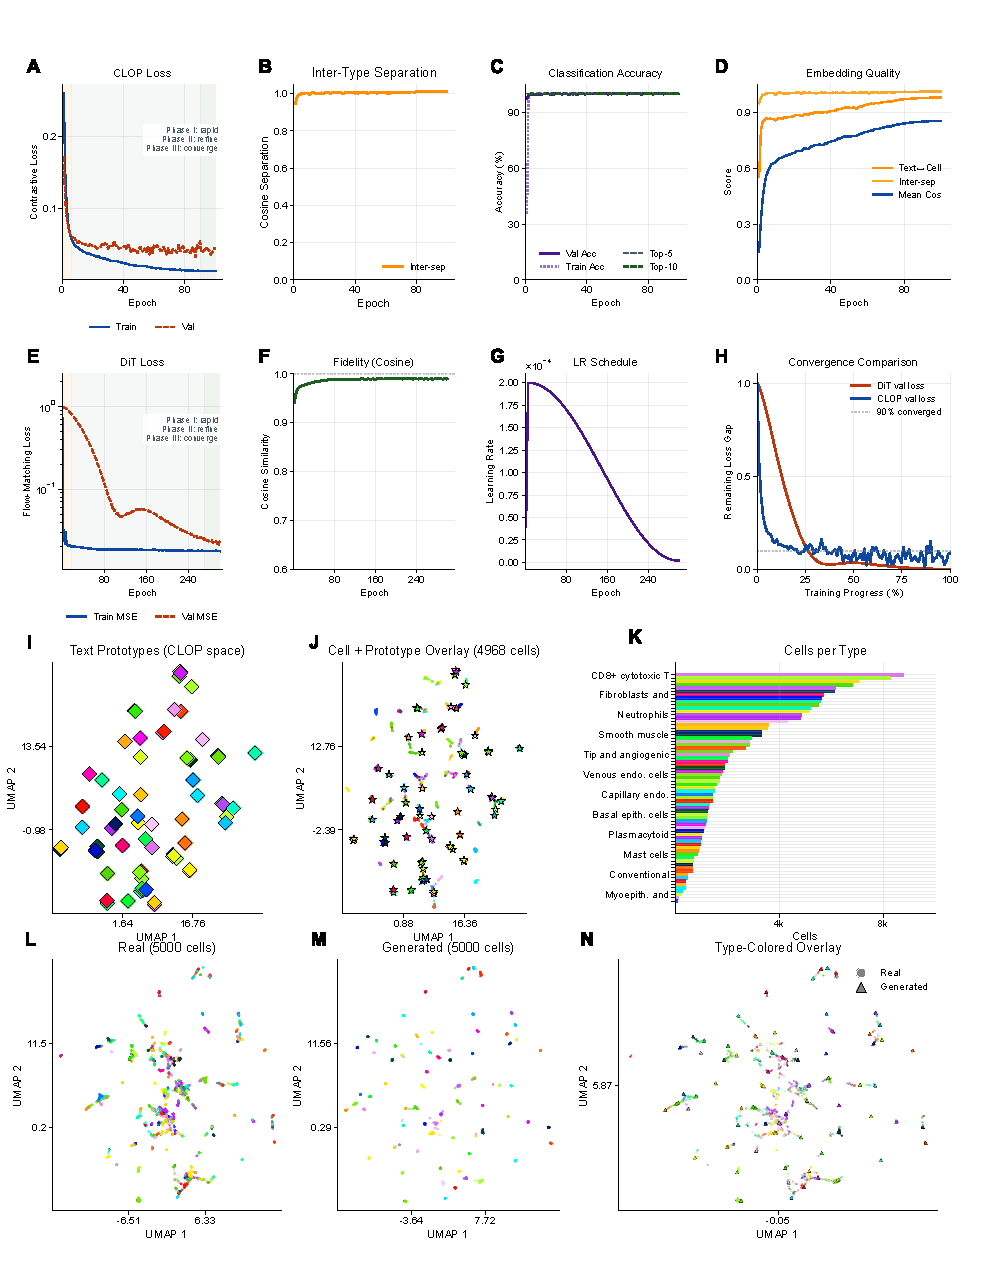
\includegraphics[width=0.95\textwidth]{Figure_02_training_embedding.pdf}
\caption{\textbf{Training dynamics and embedding space analysis.} \emph{Training dynamics} \textbf{A--D}~CLOP loss, inter-type cosine separation, batch accuracy (shown on the full 0--100\% scale to expose ceiling-like saturation of this stage-specific retrieval proxy), and embedding-quality metrics over the reported training run. \textbf{E--H}~DiT train/validation loss, velocity cosine similarity, learning-rate schedule, and normalized convergence comparison. \emph{Embedding space} \textbf{I--J}~CLOP-projected text and cell embeddings form aligned clusters in the shared space. \textbf{K}~Cell-count distribution across types. \textbf{L--N}~Real and generated scGPT embeddings occupy overlapping but distinguishable regions.\label{fig:training}\label{fig:embedding-space}}
\end{figure}

\subsection{Core Evaluation Metrics}

Table~\ref{tab:core-results} and Figure~\ref{fig:metrics} summarize performance across representative generation settings. In the high-fidelity regime (CFG = 2.0, 10-step Euler), CLOP-DiT achieves a KNN top-1 accuracy of 36.9\% ($25\times$ random chance of 1.45\%; 52 percentage points below the 89\% real-data baseline), KNN top-5 of 55.3\%, steering accuracy of 81.0\%, and linear classifier accuracy of 51.1\%. The unconditional control ($s{=}0$) collapses to chance-level type specificity (KNN = 1.0\%, steering = 47.5\%), confirming that prompt conditioning rather than the sampler or decoder alone drives the observed structure. Fr\'{e}chet distance (FD) is reported for completeness, but because it rewards global moment matching even when conditioning is ignored, we interpret it only as a secondary distributional diagnostic.

\begin{table}[!htbp]
\caption{Core evaluation results. KNN-1 and KNN-5: top-1 and top-5 $k$-nearest-neighbor accuracy among 69 deduplicated cell types (random = 1.45\%). Steering: pairwise directional accuracy (random = 50\%). DivR: diversity ratio with ideal = 1.0. LinAcc: logistic regression accuracy in embedding space (trained on real, evaluated on generated; distinct from the expression-space downstream classifier in Figure~\ref{fig:downstream-pq}). FD: Fr\'{e}chet distance~\cite{ref-fid} (lower is better, but misleading for conditional generation; see text).\label{tab:core-results}}
\begin{tabularx}{\textwidth}{lCCCCCC}
\toprule
\textbf{Method} & \textbf{KNN-1} & \textbf{KNN-5} & \textbf{Steering} & \textbf{DivR} & \textbf{LinAcc} & \textbf{FD} \\
\midrule
Real data        & 0.890 & 0.993 & ---   & 1.000 & 0.942 & 0.00 \\
CFG=2.0 Euler-10 & 0.369 & 0.553 & 0.810 & 0.513 & 0.511 & 3.17 \\
CFG=3.0 Euler-10 & 0.367 & 0.554 & 0.802 & 0.473 & 0.508 & 3.46 \\
CFG=1.0 Mid-10   & 0.288 & 0.461 & 0.807 & 0.929 & 0.357 & 2.64 \\
CFG=1.0 Euler-50 & 0.293 & 0.466 & 0.807 & 0.919 & 0.365 & 2.65 \\
CFG=0.0 (uncond) & 0.010 & 0.051 & 0.475 & 1.833 & 0.010 & 0.58 \\
Gaussian          & 0.011 & 0.048 & 0.466 & 2.277 & 0.009 & 0.03 \\
\midrule
Random chance    & 0.010 & ---   & 0.500 & ---   & ---   & ---  \\
\bottomrule
\end{tabularx}
\end{table}

\begin{figure}[!htbp]
\centering
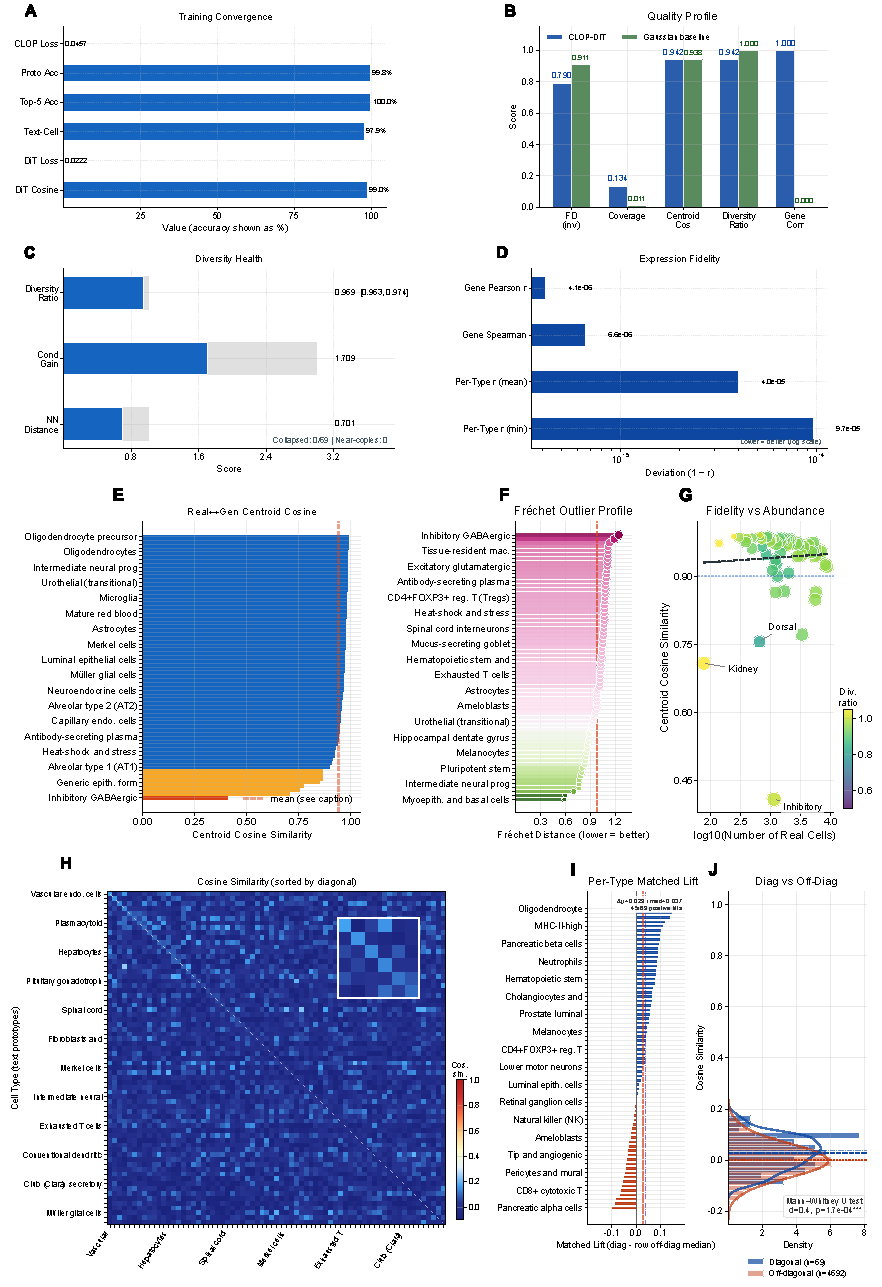
\includegraphics[width=0.84\textwidth]{Figure_03_generation_quality.pdf}
\caption{\textbf{Generation quality overview: metrics, per-type fidelity, and text--cell alignment.} \emph{Metrics dashboard} \textbf{A}~Training convergence, \textbf{B}~CLOP-DiT versus Gaussian metrics, \textbf{C}~diversity health, and \textbf{D}~expression-fidelity deviation ($1-r$, log scale). \emph{Per-type fidelity} \textbf{E}~centroid cosine by type, \textbf{F}~Fr\'{e}chet outlier profile, and \textbf{G}~abundance--fidelity scatter. \emph{Text--cell alignment} \textbf{H}~69$\times$69 text-prototype$\times$cell-centroid cosine heatmap in CLOP-projected 512-d space (mean diagonal $\mu_{\text{diag}}=0.029$; Cohen's $d=0.45$). \textbf{I}~Per-type matched lift, defined as matched text--cell similarity minus the row-wise off-diagonal median. \textbf{J}~Diagonal versus off-diagonal distributions ($\Delta=0.029$, bootstrap 95\% CI $[0.013,0.045]$, Mann--Whitney $p=1.7\times10^{-4}$).\label{fig:metrics}\label{fig:per-type-gen}\label{fig:text-cell-alignment}}
\end{figure}

\textbf{Bootstrap confidence intervals.} To quantify evaluation sampling uncertainty, we computed bootstrap 95\% CIs by resampling the 69 evaluated cell types with replacement ($B{=}1{,}000$, percentile method). All 69 deduplicated types have both real and generated cells, so the bootstrap covers the full evaluation set consistently. At an intermediate reference configuration (CFG = 1.5, Midpoint, 20 steps; selected to balance fidelity and diversity between the two primary operating points): KNN top-1 = 0.509 [0.421, 0.586], KNN top-5 = 0.728 [0.658, 0.794], steering = 1.000 [1.000, 1.000] (\textbf{ceiling effect}: all bootstrap resamples achieve perfect pairwise accuracy at this configuration, indicating that the steering metric saturates at moderate-to-high CFG and becomes non-discriminative; this ceiling limits the interpretability of steering differences across configurations), diversity ratio = 0.969 [0.963, 0.974], linear accuracy = 0.583 [0.518, 0.646], and centroid cosine = 0.898 [0.875, 0.913]. The narrow diversity ratio and centroid cosine CIs reflect uniformly high performance across types; the wider KNN CIs reflect type-dependent classification difficulty. These CIs capture evaluation sampling variability; inter-run variance across three training seeds is reported separately in Table~\ref{tab:multi-seed}.

\subsection{Multi-Seed Validation}\label{sec:multi-seed-results}

To quantify inter-run variance from stochastic initialization, data shuffling, and mini-batch ordering, we trained three independent CLOP + DiT pipelines (seeds 42, 123, 456) with identical hyperparameters and evaluated each under both operating regimes (Table~\ref{tab:multi-seed}).

\begin{table}[!htbp]
\caption{Multi-seed validation (3 independent training runs). Mean $\pm$ standard deviation for core metrics under both operating regimes. All three seeds use identical hyperparameters (Table~\ref{tab:hyperparams}), identical data splits, and identical evaluation protocol.\label{tab:multi-seed}}
\centering
\small
\begin{tabular}{lcccc}
\toprule
 & \multicolumn{2}{c}{\textbf{High-Fidelity (CFG=2.0, Euler)}} & \multicolumn{2}{c}{\textbf{High-Diversity (CFG=1.0, Midpoint)}} \\
\cmidrule(lr){2-3}\cmidrule(lr){4-5}
\textbf{Metric} & \textbf{Mean $\pm$ Std} & \textbf{Range} & \textbf{Mean $\pm$ Std} & \textbf{Range} \\
\midrule
KNN Top-1      & $0.348 \pm 0.082$ & [0.258, 0.419] & $0.273 \pm 0.048$ & [0.220, 0.312] \\
KNN Top-5      & $0.535 \pm 0.016$ & [0.524, 0.553] & $0.465 \pm 0.038$ & [0.430, 0.504] \\
Steering       & $0.808 \pm 0.009$ & [0.798, 0.817] & $0.801 \pm 0.008$ & [0.792, 0.807] \\
Diversity Ratio & $0.511 \pm 0.015$ & [0.496, 0.525] & $0.924 \pm 0.016$ & [0.906, 0.937] \\
Linear Acc.    & $0.488 \pm 0.023$ & [0.465, 0.511] & $0.355 \pm 0.097$ & [0.257, 0.452] \\
Centroid Cos.  & $0.892 \pm 0.012$ & [0.878, 0.900] & $0.892 \pm 0.010$ & [0.880, 0.898] \\
\bottomrule
\end{tabular}
\end{table}

Inter-run standard deviations are small relative to effect sizes: steering accuracy varies by $< 1$ percentage point ($\sigma = 0.009$), diversity ratio by $< 2$ percentage points ($\sigma = 0.015$--$0.016$), and centroid cosine by $\sim 1\%$ ($\sigma = 0.010$--$0.012$). KNN top-1 accuracy exhibits the largest inter-seed variance ($\sigma = 0.082$ in the high-fidelity regime), reflecting the sensitivity of nearest-neighbor classification to the decision boundary in the tightly-packed scGPT embedding space. Critically, the qualitative conclusions---$25\times$ above random chance, $\sim$52-point gap from real data, near-ideal diversity at CFG\,=\,1.0---are stable across all three seeds.

\subsection{Per-Type Generation Quality and Text--Cell Alignment}\label{sec:per-type}

Beyond aggregate metrics, per-type analysis reveals which cell types benefit most from text conditioning and where failures concentrate. Figure~\ref{fig:per-type-gen} presents per-type generation quality and text--cell alignment. The enhanced per-type analysis now makes heterogeneity explicit: centroid cosine is ranked across all 69 deduplicated cell types; the Fr\'echet profile highlights outlier types rather than only reporting the mean, and the abundance--fidelity scatter encodes Fr\'echet distance as bubble size and diversity ratio as color. This reveals that failure modes are concentrated in a small subset of cell types with high intrinsic within-type heterogeneity rather than being uniform across the atlas. We replace the qualitative phrase ``biologically difficult'' with an operational definition: cell types with broad intrinsic within-type heterogeneity, quantified as \texttt{real\_intra\_cos} below the 25th percentile. Across the 68 matched cell types, per-type Fr\'echet distance is only weakly related to training-set abundance (Spearman $\rho = 0.57$, $p = 4.9\times10^{-7}$) but is strongly explained by within-type heterogeneity ($\rho = -0.77$, $p = 3\times10^{-13}$). A bottom-quartile-by-training-count slice does not show a fidelity gap (centroid cosine 0.907 vs.\ 0.896 for the top quartile, Mann--Whitney $p = 0.02$, favouring the underrepresented set). Within-type heterogeneity is therefore the better-targeted diagnosis.

\textbf{KNN error composition.} Using a 10-family biologically grounded taxonomy over the 69 evaluation cell types, 49.2\% of all KNN mis-typings stay within the same cell-lineage family---about half of the reported errors are graceful degradations between closely related cell types rather than catastrophic cross-lineage failures. Of the top-15 most-confused cell-type pairs, 9 are within-family (e.g., pancreatic $\delta$~$\leftrightarrow$~neuroendocrine; tissue-resident macrophages~$\leftrightarrow$~MHC-II\textsuperscript{+} antigen-presenting cells; fibroblasts~$\leftrightarrow$~mesenchymal stem cells), and the 6 cross-family pairs are dominated by functional-state overlap or well-known shared-marker confusions. Every family achieves within-family accuracy $\geq 0.94$ except the proliferation/stress/pluripotent family, which cuts across lineages by definition. The full family-by-family error matrix is provided in Figure~\ref{fig:knn-family-heatmap} (Appendix~\ref{app:suppl-figs}).

\textbf{Species stratification.} Stratifying all headline per-type metrics by organism yields 18 human-only, 8 mouse-only, and 43 dual-organism cell types. Across human-only and mouse-only types, the two groups are statistically indistinguishable on centroid cosine (0.917 vs.\ 0.919, Mann--Whitney $p = 0.14$), Fr\'echet distance (1.052 vs.\ 1.028, $p = 0.85$), diversity ratio ($p = 0.18$), expression Pearson $r$ ($p = 0.43$), and real within-type cosine tightness ($p = 0.87$). The $59/21$ dataset-count imbalance does not propagate to evaluation-level species bias at the type level. Per-metric distributions by organism group are visualised in Figure~\ref{fig:organism-stratified} (Appendix~\ref{app:suppl-figs}).

The text--cell alignment analysis (panels H--J; Figure~\ref{fig:text-cell-alignment}) should be read as a condition-space diagnostic rather than as a direct generated-cell accuracy metric. In the CLOP-projected space, matched text prototypes show a small but statistically significant diagonal lift over off-diagonal cell-type centroids (mean diagonal--off-diagonal difference $=0.029$, bootstrap 95\% CI $[0.013,0.045]$, Mann--Whitney $p=1.7\times10^{-4}$). This supports functional text--cell coupling, while its modest absolute cosine scale is consistent with the tightly packed scGPT geometry and is therefore interpreted alongside the generation-side KNN, steering, and centroid-cosine metrics rather than in isolation.

\subsection{Gene-Level Fidelity}

A key question for conditional generation is whether cell-type-specific marker gene signatures and gene-level expression statistics are preserved. Figure~\ref{fig:gene-fidelity} addresses this at two levels: marker-gene comparison (top) confirms that CLOP-DiT preserves cell-type-specific expression signatures, while per-gene correlation analysis (bottom; Figure~\ref{fig:expr-corr}) localizes fidelity in gene-wise means and marker-level residuals through per-gene mean scatters and residual distributions. Figure~\ref{fig:expr-analysis} provides a broader view of expression distribution properties, including per-gene coefficient of variation and per-cell variability.

\textbf{Quantitative variance summary.} Across the 1{,}790 genes scored in the in-distribution evaluation, 85\% fall inside the $[0.5, 2.0]$ tolerance band for the generated/real variance ratio, with a median standard-deviation ratio of 1.33 and a pooled gene-wise variance Pearson correlation of $r_\text{var} = 0.988$. Restricting to within-type variance, median $r_\text{var}$ across the 69 cell types is $+0.85$ and 100\% of types exhibit a positive correlation, with 75\% of (type, gene) pairs inside tolerance and 8.7\% showing a variance deficit greater than two-fold. The cross-dataset held-out evaluation remains the stricter test and continues to show variance collapse (median ratio 0.01--0.02).

\begin{figure}[!htbp]
\centering
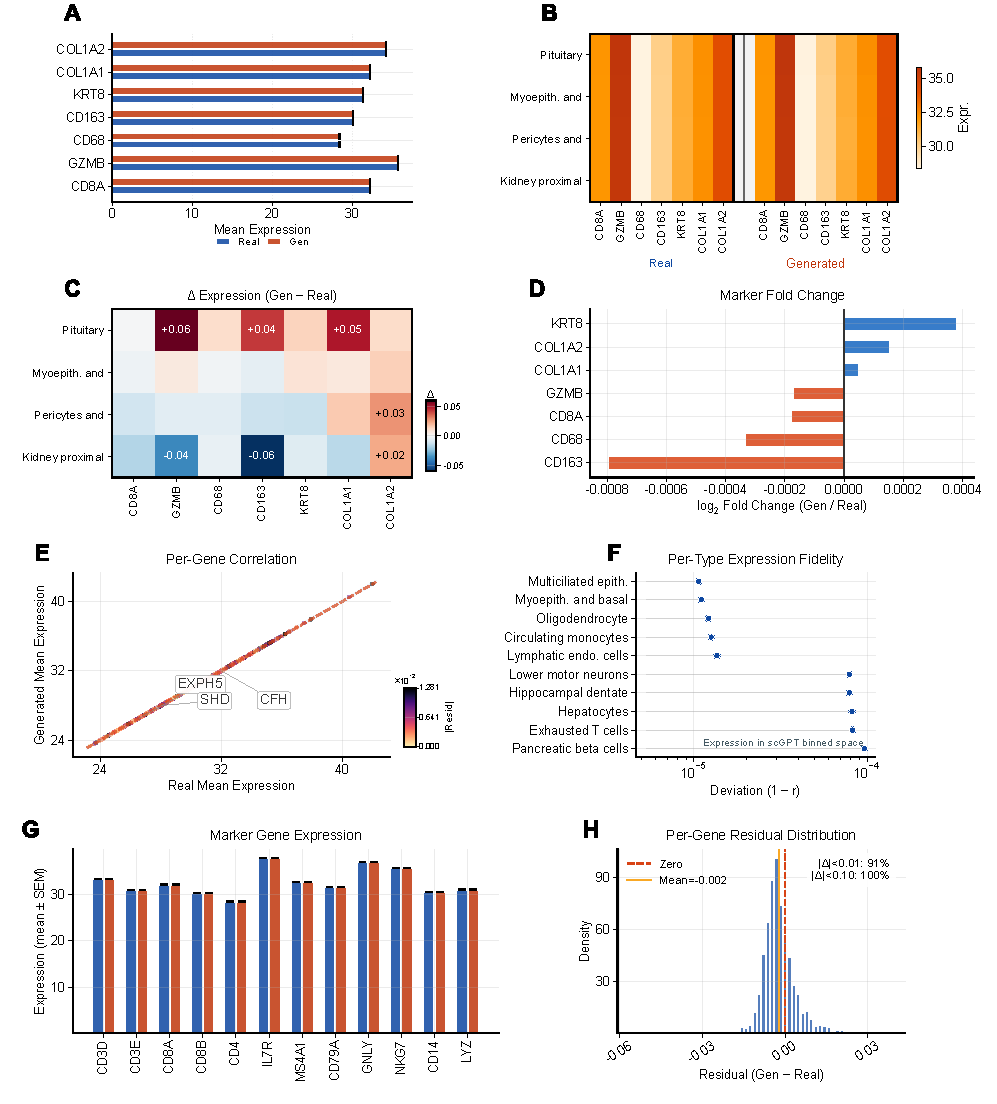
\includegraphics[width=0.95\textwidth]{Figure_04_gene_fidelity.pdf}
\caption{\textbf{Gene-level fidelity analysis.} \textbf{A}~Paired bar chart of canonical marker-gene expression in real vs.\ generated cells. \textbf{B}~Per-type $\times$ marker dual heatmap. \textbf{C}~Difference heatmap ($\Delta$ = generated $-$ real). \textbf{D}~Log$_2$ fold-change summary across the marker panel. \textbf{E}~Per-gene mean-expression scatter with residual coloring and short callouts for the largest outliers. \textbf{F}~Per-type deviation from perfect correlation ($1-r$, log scale). \textbf{G}~Marker-gene expression comparison with error whiskers. \textbf{H}~Per-gene residual distribution.\label{fig:gene-fidelity}\label{fig:markers}\label{fig:expr-corr}}
\end{figure}

\vspace{-0.5em}
\begin{figure}[!htbp]
\centering
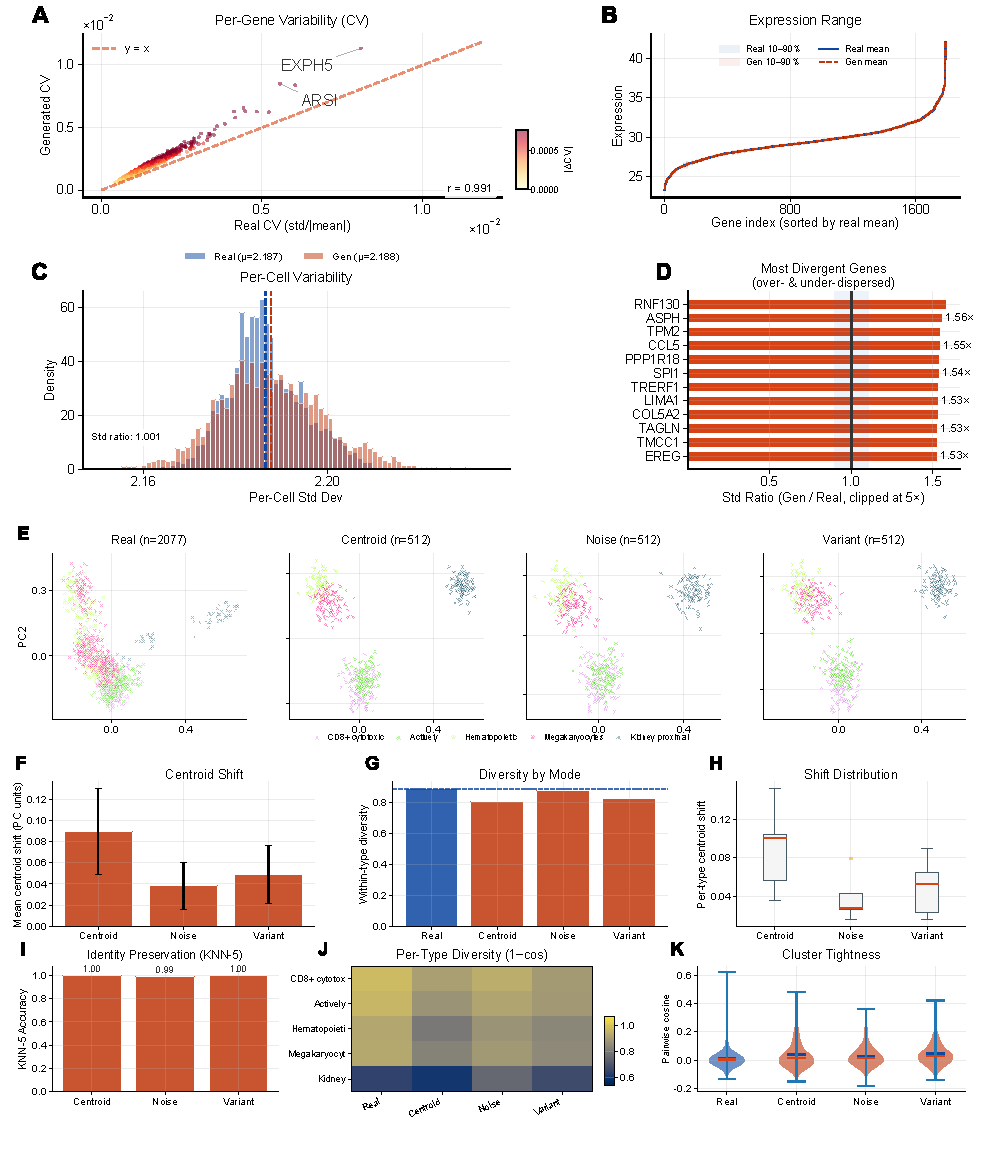
\includegraphics[width=0.95\textwidth]{Figure_05_expression_conditioning.pdf}
\caption{\textbf{Expression distribution analysis and conditioning landscape.} \textbf{A}~Per-gene coefficient-of-variation scatter (real vs.\ generated) with compact outlier callouts placed near their points. \textbf{B}~Expression-range ribbons. \textbf{C}~Per-cell variability distributions. \textbf{D}~Top variable genes ranked by standard-deviation ratio. \textbf{E}~PCA projection of real and generated cells under three conditioning modes (centroid, noisy, variant), with the shared cell-type legend placed beneath the scatter row. \textbf{F}~Mean centroid shift per mode. \textbf{G}~Within-type diversity by mode relative to the real baseline. \textbf{H}~Per-type centroid shift distributions. \textbf{I}~KNN-5 identity-preservation accuracy. \textbf{J}~Per-type diversity heatmap ($1 - \text{mean cosine}$). \textbf{K}~Pairwise cosine distributions comparing cluster tightness across modes.\label{fig:expr-analysis}\label{fig:cond-umap}}
\end{figure}

\subsection{Conditioning Landscape and Diversity Trade-Offs}

\noindent After establishing headline fidelity metrics, we next ask how controllable the generator is and how much diversity is sacrificed as guidance increases.

Figure~\ref{fig:cond-umap} shows that CLOP conditions occupy a well-separated landscape in projection space and that generated latent clouds follow this organization, enabling interpretable control over cell-type identity. Together with Figures~\ref{fig:diversity} and~\ref{fig:expr-diversity}, this section therefore serves as the main robustness analysis for whether stronger steering can be achieved without erasing biologically meaningful heterogeneity.

Figure~\ref{fig:diversity} breaks this trade-off into interpretable diagnostics rather than a single scalar summary. Most cell types remain under-dispersed relative to real data, yet nearest-neighbour distances stay above the memorization threshold. Increasing classifier-free guidance monotonically contracts within-type spread, whereas adding conditioning noise partially restores diversity without destroying centroid alignment. The practical outcome is a two-regime operating envelope: stronger guidance improves type fidelity, while Midpoint sampling at CFG = 1.0 best preserves expression-level diversity (Figure~\ref{fig:expr-diversity}) and yields the most balanced gene-level variance profile. The combined diversity diagnostic suite (Figure~\ref{fig:diversity-suite}, panels~A--D) and the dedicated noise-scale sweep (Figure~\ref{fig:noise-tradeoff}, panel~E) jointly characterise the CFG contraction and the $\varepsilon = 0.03$ sweet-spot region used in production.

\begin{figure}[!htbp]
\centering
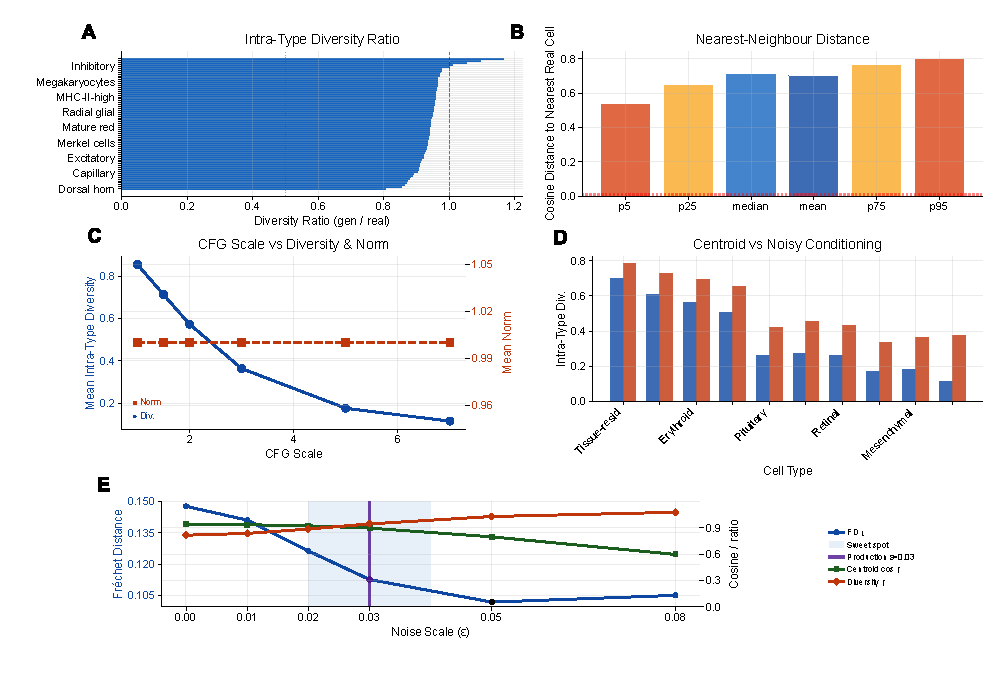
\includegraphics[width=0.95\textwidth]{Figure_06_diversity_diagnostics.pdf}
\caption{\textbf{Diversity diagnostics and noise-scale trade-off.} \textbf{A}~Intra-type diversity ratio (generated/real) ranked across cell types; the dashed line marks the ideal ratio of 1.0. \textbf{B}~Percentiles of the cosine distance from each generated cell to its nearest real-cell neighbour; the dotted line marks the memorization threshold. \textbf{C}~Classifier-free-guidance (CFG) scale versus mean intra-type diversity and mean latent norm. \textbf{D}~Per-type intra-type diversity under centroid-only versus centroid+noise conditioning. \textbf{E}~Noise-scale sweep showing Fr\'{e}chet distance, centroid cosine, and diversity ratio as functions of $\varepsilon$; the shaded band marks the sweet-spot region and the vertical line marks the production configuration ($\varepsilon = 0.03$).\label{fig:diversity-suite}\label{fig:diversity}\label{fig:noise-tradeoff}}
\end{figure}

\begin{figure}[!htbp]
\centering
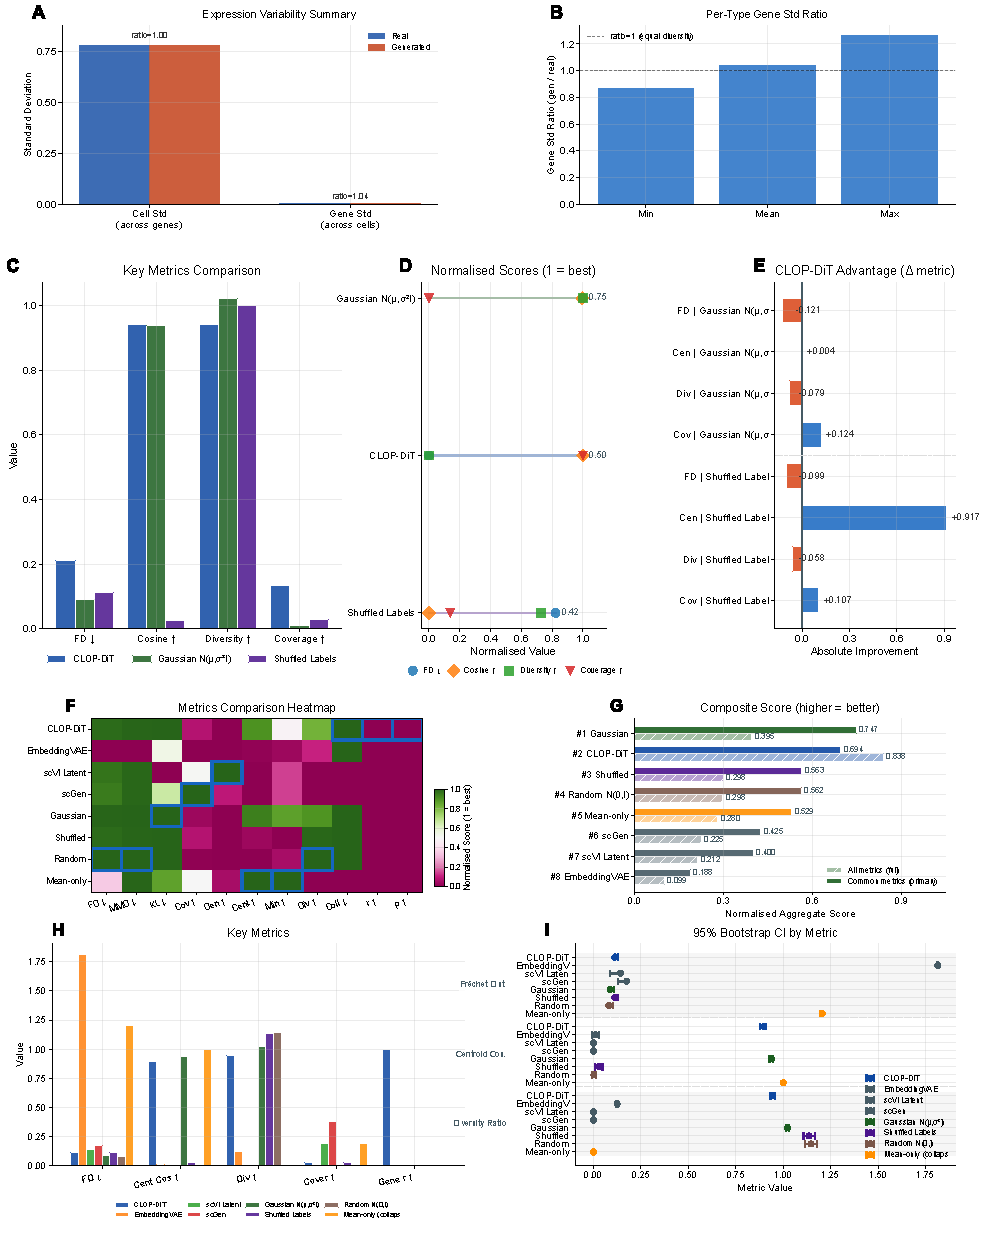
\includegraphics[width=0.95\textwidth]{Figure_07_baseline_benchmark.pdf}
\caption{\textbf{Expression-level diversity, baseline comparison, and composite benchmark.} \textbf{(Top)} \textbf{A}~Gene-expression variability summary (real vs.\ generated). \textbf{B}~Per-type gene standard-deviation ratio. \textbf{(Middle)} \textbf{C}~Head-to-head grouped-bar analysis across four evaluation metrics. \textbf{D}~Ranked normalised scores per method. \textbf{E}~Absolute metric delta of CLOP-DiT relative to each baseline. \textbf{(Bottom)} \textbf{F}~Normalized metrics heatmap (methods $\times$ metrics). \textbf{G}~Composite score (solid = common-metrics-only; hatched = full). \textbf{Warning: the full composite is structurally biased}; the common-metrics-only bars are the fair comparison. \textbf{H}~Grouped comparison of four interpretable metrics. \textbf{I}~95\% bootstrap confidence intervals.\label{fig:expr-diversity}\label{fig:baselines}\label{fig:benchmark}}
\end{figure}

\subsection{Baseline Comparison and Composite Benchmark}

\noindent We benchmark CLOP-DiT against both simple parametric controls (Gaussian per-type sampling, shuffled-label controls, mean-collapse baselines) and learned generative models (scVI Latent, scGen, EmbeddingVAE).

CLOP-DiT is compared against unconditional generation (CFG = 0), Gaussian sampling from per-type statistics, shuffled-label and mean-collapse controls, EmbeddingVAE, scVI Latent~\cite{ref-scvi}, and a conditional scGen baseline~\cite{ref-scgen} implemented as conditional scVI with cell-type covariates. Figure~\ref{fig:baselines} reveals a consistent pattern: CLOP-DiT is strongest on conditioning-sensitive and downstream-relevant metrics, especially steering and classifier transfer, whereas unconditional or weakly conditioned baselines can score better on FD-like objectives because those metrics reward global moment matching even when cell-type steering is absent.

Figure~\ref{fig:benchmark} aggregates these results into a composite score across eight methods. \textbf{On the nine distributional metrics shared by all methods---the primary fair comparison---the Gaussian baseline (0.747) slightly exceeds CLOP-DiT (0.694)}, showing that simple mean-matching approaches remain competitive when evaluation ignores condition-sensitive biology. The scGen baseline (common-metrics composite 0.425) achieves the best \emph{coverage} among the learned baselines (0.384 vs.\ 0.028 for CLOP-DiT), reflecting the flexibility of its label-conditioned VAE latent space. When the eight downstream biology metrics reported only by CLOP-DiT are included, the full composite rises to 0.838 versus 0.395 for Gaussian and 0.225 for scGen; however, this full score is structurally biased in favor of CLOP-DiT and \textbf{should not be used for method ranking}. We therefore treat the common-metrics-only composite as the main benchmark and the full composite as a supplementary capability summary.

\subsection{Downstream Biological Validation}

Beyond distributional metrics, we evaluate whether generated cells are usable in standard single-cell analysis workflows. These analyses are implemented from matched real/generated AnnData objects with shared preprocessing and use Scanpy~\cite{ref-scanpy} for the single-cell workflow, ensuring that any downstream advantage is not caused by mismatched feature engineering. Two downstream tasks are assessed on real and generated cells jointly:

\textbf{Clustering, mixing, and classifier alignment} (Figure~\ref{fig:downstream-pq}): We construct matched AnnData objects from real and generated expression matrices, select 2,000 shared highly variable genes, perform PCA and Leiden~\cite{ref-leiden} clustering on the combined dataset, and compute the Adjusted Rand Index (ARI), Normalized Mutual Information (NMI), cluster purity, and per-type KNN mixing scores~\cite{ref-integration-benchmark}. High mixing scores indicate that generated cells partially co-localize with real cells of the same type in the joint embedding, though the discriminator AUC of 0.656 confirms that real and generated populations remain distinguishable. A logistic regression classifier is trained on real PCA embeddings to predict cell type, then evaluated on generated embeddings to measure transfer accuracy and macro-F1. The enhanced classifier panel reports a per-type precision/recall/F1 heatmap in addition to the confusion matrix and discriminator ROC, demonstrating that downstream performance exhibits strong heterogeneity across cell types. The real-vs.-generated discriminator AUC (0.656) indicates partial but non-trivial separability, so downstream usability remains qualified rather than near-indistinguishable transfer. Complementary feature-importance panels (Figure~\ref{fig:discriminator} in Appendix~\ref{app:suppl-figs}) show that discriminator separability is primarily mean-driven ($|r| = 0.67$), weight-concentrated (Gini = 0.42), and type-heterogeneous (mean per-type AUC = 0.92).

\textbf{DE concordance} (Figure~\ref{fig:downstream-r}): Wilcoxon rank-sum differential expression analysis~\cite{ref-wilcoxon} is performed on three biologically meaningful contrasts (CD8 vs.\ CD4 T cells, resident macrophage vs.\ monocyte, epithelial tumor vs.\ fibroblast). We compare log-fold changes between real and generated data via Pearson and Spearman correlations, Jaccard overlap of the top-50 DE genes, and sign-agreement fractions. The enhanced DE figure weights each gene by effect size and colors it by adjusted significance, which separates minor noisy disagreements from the biologically important genes that dominate each contrast.

\begin{figure}[!htbp]
\centering
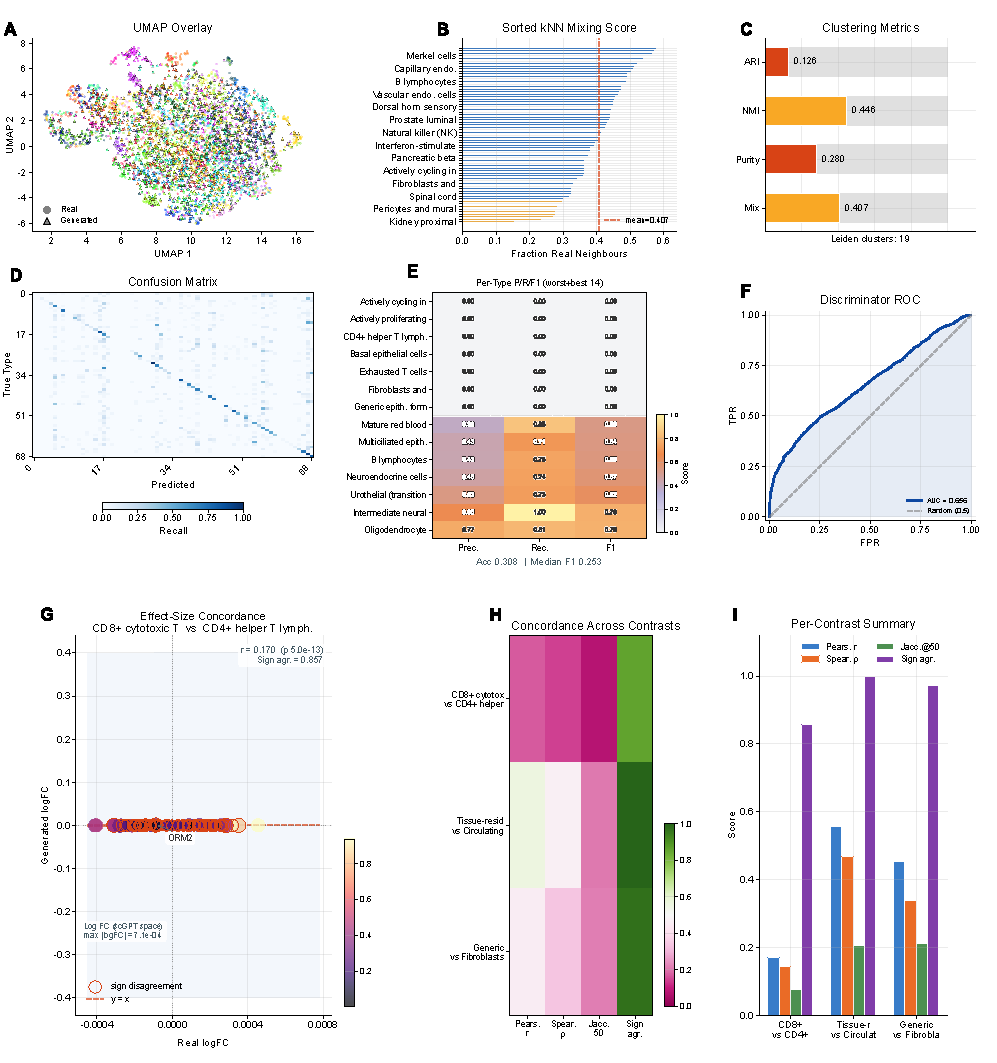
\includegraphics[width=0.95\textwidth]{Figure_08_downstream_validation.pdf}
\caption{\textbf{Downstream validation.} \textbf{(Top)} \textbf{A}~Leiden clustering on combined real + generated data with UMAP overlay, \textbf{B}~sorted per-type KNN mixing profile, and \textbf{C}~compact cluster-alignment gauges (ARI, NMI, cluster purity, mean KNN mixing). \textbf{D}~Cell-type classification confusion matrix, \textbf{E}~precision/recall/F1 heatmap, and \textbf{F}~real-vs.-generated discriminator ROC curve. \textbf{(Bottom)} \textbf{G}~Effect-size-weighted logFC scatter for the leading contrast; sign-disagreement genes are outlined. \textbf{H}~Concordance heatmap (Pearson~$r$, Spearman~$\rho$, Jaccard@50, sign agreement) across three contrasts. \textbf{I}~Per-contrast grouped-bar summary. Effect sizes in panel \textbf{G} are in scGPT latent space (max $|\text{logFC}| \approx 7\times10^{-4}$), not raw transcript counts.\label{fig:downstream-pq}\label{fig:downstream-r}}
\end{figure}
Together, these results establish that CLOP-DiT generates text-conditioned single-cell profiles with measurable type specificity, though with performance trade-offs between fidelity and diversity that depend on the operating regime.

\subsection{In-Distribution Expression-Level Validation}\label{sec:cross-dataset}

To assess biological fidelity across tissue contexts, we performed expression-level validation on five datasets (Table~\ref{tab:s4_biovalidation}) spanning lung adenocarcinoma (GSE123902), basal cell carcinoma (GSE123813), liver T-cell hepatocellular carcinoma (GSE98638), gastric cancer (GSE183904), and acute lymphoblastic leukemia in bone marrow (GSE132509). Four of these five datasets (GSE123902, GSE123813, GSE98638, GSE132509) are from the training split; only GSE183904 is among the 8 held-out validation studies (Table~\ref{tab:s2_validation}). This analysis therefore primarily evaluates in-distribution gene-level reconstruction fidelity rather than out-of-distribution generalization. For each dataset, cells were generated conditioned on the dataset-specific text descriptions and compared with real (scGPT-reconstructed) expression profiles; because both the generated and reference expressions are decoded by the same frozen scGPT decoder, the resulting correlations measure decoder-reconstructed fidelity rather than agreement with raw sequencing counts. Per-gene mean expression, gene-level variance, and Fr\'{e}chet distance in both gene space and embedding space were computed for each dataset independently (Table~\ref{tab:cross-dataset}).

\begin{table}[!htbp]
\caption{Cross-dataset biological validation (decoder-reconstructed fidelity). Per-gene mean expression Pearson correlation ($r$) and coefficient of determination ($R^2$), gene variance Pearson correlation ($r_\text{var}$), and Fr\'{e}chet distance in PCA-50 gene space (FD\textsubscript{gene}) and scGPT embedding space (FD\textsubscript{embed}) for real and generated cells. Both ``real'' and generated expression profiles are decoded by the same frozen scGPT decoder; correlations therefore measure decoder-reconstruction consistency rather than agreement with raw sequencing counts. Split indicates whether the dataset was used for training (Train) or held-out validation (Val). All five datasets achieve gene\_mean $r > 0.999$.\label{tab:cross-dataset}}
\centering
\small
\begin{tabular}{lccccccc}
\toprule
\textbf{Dataset (GEO)} & \textbf{Tissue} & \textbf{Split} & \textbf{$r_\text{mean}$} & \textbf{$R^2$} & \textbf{$r_\text{var}$} & \textbf{FD\textsubscript{gene}} & \textbf{FD\textsubscript{embed}} \\
\midrule
GSE123902 & Lung     & Train & 0.9995 & 0.9990 & $+$0.011  & $3.07 \times 10^{-5}$ & 73.9 \\
GSE123813 & Skin (BCC)  & Train & 0.9997 & 0.9995 & $-$0.019  & $5.25 \times 10^{-6}$ & 72.7 \\
GSE98638  & Liver    & Train & 0.9995 & 0.9989 & $-$0.003  & $2.04 \times 10^{-5}$ & 155.4 \\
GSE183904 & Gastric  & Val & 0.9997 & 0.9994 & $+$0.013  & $1.30 \times 10^{-5}$ & 62.1 \\
GSE132509 & Blood (ALL)  & Train & 0.9993 & 0.9985 & $-$0.007  & $8.87 \times 10^{-6}$ & 69.1 \\
\bottomrule
\end{tabular}
\end{table}

Across all five datasets, per-gene mean expression Pearson correlation exceeds 0.999 and $R^2$ exceeds 0.998. Because both reference and generated profiles pass through the same frozen scGPT decoder, these correlations reflect decoder-reconstructed fidelity rather than absolute biological accuracy against raw counts. However, per-gene variance correlation ($r_\text{var}$) is near zero across all datasets (range: $-0.019$ to $+0.013$), indicating that the model reproduces mean expression accurately but does not preserve gene-level variability---consistent with the flow-matching mean-regression bias. Embedding-space FD (62.1--155.4) is substantially higher than gene-space FD ($<10^{-4}$), reflecting the many-to-one decoder mapping.

\textbf{Baselines for gene-wise variance recovery.} To contextualise the near-zero cross-dataset $r_\text{var}$, we bracket CLOP-DiT between two Gaussian reference generators. At the CLOP latent scale, CLOP-DiT recovers within-type variance structure with a mean across-type Pearson $r_\text{var}$ of $+0.201$, sitting strictly between a type-agnostic pooled-Gaussian floor ($+0.014$, only 60.9\% of types above zero) and a type-aware Gaussian oracle that matches real per-type $\mu, \Sigma$ exactly ($+0.813$). At the decoded-expression scale, pooled $r_\text{var}$ converges to $>0.98$ for all three generators because HVGs dominate gene-wise variance; the discriminating statistic is the within-type pooled median variance ratio (0.94 for the type-aware oracle, 1.13 for CLOP-DiT, 1.79 for the pooled Gaussian). The near-zero cross-dataset variance ratio is therefore not a shared feature of latent-generation pipelines; CLOP-DiT under-represents within-type variance relative to the type-aware oracle, consistent with the upstream latent-compression mechanism. Importantly, the cross-dataset variance deficit and the in-distribution Gaussian advantage address different research questions (decoder fidelity vs.\ type-level distributional matching), so these two findings should not be conflated in composite benchmark comparisons.

\subsection{CLOP Ablation Study}\label{sec:ablation}

To validate the contribution of individual CLOP components, we conducted 15 ablation experiments, removing or modifying one component at a time while holding all other settings constant. Table~\ref{tab:ablation} summarizes the six most informative ablations.

\begin{table}[!htbp]
\caption{CLOP ablation study (\textbf{ablation baseline only}; not the final production model). Validation prototype accuracy (top-1) for the ablation baseline configuration (all features enabled) and representative ablations. $\Delta$~denotes the change from baseline in percentage points. These results characterize the CLOP alignment stage in isolation and do not directly predict downstream DiT generation quality; the final production model uses different regularization settings.\label{tab:ablation}}
\centering
\small
\begin{tabular}{llcc}
\toprule
\textbf{Ablation} & \textbf{Category} & \textbf{Val Proto Acc (\%)} & \textbf{$\Delta$ (pp)} \\
\midrule
$-$cohesion        & regularization & 86.41 & $+$10.24 \\
$-$cell noise      & regularization & 86.23 & $+$10.07 \\
$-$dropout (lighter) & regularization & 77.32 & $+$1.15 \\
Baseline           & reference      & 76.17 & --- \\
Fixed temperature   & optimization   & 71.55 & $-$4.61 \\
High variant prob   & regularization & 70.14 & $-$6.03 \\
\bottomrule
\end{tabular}
\end{table}

The two most impactful ablations are cohesion regularization removal ($+$10.24~pp) and cell noise augmentation removal ($+$10.07~pp), both of which improve prototype accuracy. This counterintuitive result has the following mechanistic explanation: both cohesion loss and cell noise augmentation act as within-group tightening forces that penalize intra-cluster variance. In a contrastive learning regime where the primary bottleneck is inter-group separation (raw pairwise cosine 0.994), these tightening forces compete with the alignment gradient rather than complementing it. In effect, the network spends representational capacity enforcing tight within-group clusters before inter-group margins have been established, diverting training signal from the discrimination task. Removing these terms allows the optimizer to focus more directly on inter-group separation, the dominant constraint in this Stage-1 diagnostic. This interpretation is consistent with recent analyses of regularization--discrimination trade-offs in contrastive learning~\cite{ref-siglip}. Architecture ablations (projection dimension 256 vs.\ 512 vs.\ 768) have minimal impact (within $\pm$0.3~pp), indicating that the CLOP aligner is not sensitive to projection dimension in this range. Fixed temperature ($-$4.61~pp) and high variant probability ($-$6.03~pp) degrade performance substantially relative to the ablation baseline (which used a learnable temperature). \textbf{Clarification:} The ablation baseline used a learnable $\tau$, whereas the final production model uses fixed $\tau = 14.0$ in combination with a stratified validation split (Section~\ref{sec:dataset}). The production configuration was selected based on the full-pipeline generation quality assessment, not solely on CLOP prototype accuracy; the ablation table characterizes the CLOP alignment stage in isolation and does not directly predict downstream DiT generation performance.

\textbf{Stage-1 to full-pipeline transfer (partial-reversal caveat).} To quantify how well Stage-1 CLOP ablation rankings predict end-to-end generation quality, we retrained the full DiT on top of three CLOP variants (ablation-baseline, $-$cohesion, $-$cell-noise) and regenerated 6{,}900 embeddings per variant. The Stage-1 ranking is a partial-reversal proxy: the $-$cohesion arm reaches the highest Stage-1 prototype accuracy (0.864 vs.\ 0.762 baseline, $+10.2$\,pp) yet becomes the weakest end-to-end generator, degrading Frechet distance to 0.230 (vs.\ 0.175 baseline, $+31\%$), coverage to 0.079 (vs.\ 0.144, $-45\%$), and per-type centroid cosine to 0.854 (vs.\ 0.929, $-8.1$\,pp). The $-$cell-noise variant transfers only partially (FD $0.145$, centroid cosine $0.923$). A Stage-1 projected-text diagnostic confirms that the production and ablation CLOPs learn structurally unrelated inter-type geometries (inter-type-similarity matrix Pearson $r = 0.04$--$0.06$). CLOP ablation rankings should therefore be read as a characterisation of the aligner's loss landscape rather than as a predictor of end-to-end generation quality. The formal ZCA ablation (Table~\ref{tab:zca-ablation}) spans three matched CLOP training runs --- full ZCA, mean-centring + L2 normalisation only, and no preprocessing --- with composite alignment quality dropping by only $1.0\%$ across the full ablation; ZCA's principal measurable contribution is a $+5\%$ improvement in positive-pair cosine similarity (0.851 vs.\ 0.809), reflecting decorrelation rather than structural alignment gain.

\begin{table}[!htbp]
\caption{ZCA whitening ablation (three matched CLOP training runs). Composite CLOP quality, positive-pair cosine similarity, CLOP prototype accuracy (top-1), and downstream DiT KNN accuracy at CFG~=~2.0 across full ZCA, centring + L2 only, and no preprocessing.\label{tab:zca-ablation}}
\centering
\small
\begin{tabular}{lcccc}
\toprule
\textbf{Configuration} & \textbf{CLOP Quality} & \textbf{Pos-pair cos} & \textbf{Proto Acc (\%)} & \textbf{DiT KNN (\%)} \\
\midrule
With ZCA (production) & 0.966 & 0.851 & 76.17 & 36.9 \\
Centre + L2 only & 0.960 & 0.815 & 76.03 & --- \\
Without preprocessing & 0.956 & 0.809 & 75.42 & 36.5 \\
\bottomrule
\end{tabular}
\end{table}

\subsection{Rare Cell Augmentation}\label{sec:rare-cell}

In a pilot augmentation experiment, we evaluated whether generated cells can improve classifier performance on underrepresented types. Augmentation of ``Cycling cells'' ($<$5\% prevalence) at 1--10$\times$ ratios did not improve Cycling-cell F1 (baseline 0.828 $\to$ 0.741--0.786 after augmentation), though overall macro F1 remained stable (0.947--0.964).

\textbf{Failure mechanism.} Decomposing within-type variance at the latent and expression scales attributes this failure to upstream latent under-dispersion rather than downstream decoder collapse. Across the 18 lowest-abundance cell types, the generator produces latents whose within-type total variance is 30--66\% of real (median $0.50\times$ real), yet the scGPT decoder recovers expression-space variance to 47--190\% of real (median $1.07\times$ real). For the Cycling population, latent and expression total variance are within 5--15\% of real, but intra-cluster cosine similarity is $4.6\times$ higher in generated samples, indicating highly directional synthetic diversity.

\textbf{Systematic augmentation-strategy sweep.} A $2\times 6\times 4$ sweep over two rare cell types (Megakaryocytes, Ameloblasts) $\times$ six augmentation strategies (no augmentation, random oversampling, SMOTE, CLOP-DiT, CLOP-DiT + oversampling, CLOP-DiT + SMOTE) $\times$ four ratios ($1\times$, $2\times$, $5\times$, $10\times$) confirms that no strategy improves rare-class F1 over the no-augmentation baseline (Megakaryocytes baseline F1 $= 0.917$; Ameloblasts $= 0.937$). Classical methods degrade monotonically with ratio (random oversampling $\to 0.807/0.859$ at $10\times$; SMOTE $\to 0.833/0.879$) while CLOP-DiT-only stays flat ($0.917/0.929$ at $10\times$). This is the expected consequence of the centroid-biased latent structure: additional synthetic samples match the type centroid but do not add the heterogeneity needed to shift the decision boundary. Future augmentation work is therefore directed at generator-side heterogeneity objectives, not downstream mixing strategies.

\textbf{Forced-scarcity rescue.} To verify that the B3 null result is not a ceiling artefact (baseline F1 $\geq 0.92$ leaves little headroom for augmentation to exploit), we repeated the sweep after artificially reducing each rare class to 30 training cells, which drops baseline F1 to $\approx 0.50$ on both Megakaryocytes and Ameloblasts. Under genuine scarcity, augmentation recovers substantially: random oversampling reaches $0.783/0.866$ at $10\times$, SMOTE reaches $0.769/0.834$, CLOP-DiT-only reaches $0.719/0.670$, and the hybrid CLOP-DiT + oversampling strategy reaches $0.772/0.835$. Oversampling is strongest at the embedding level because duplicating real points reinforces the correct centroid for a logistic classifier; CLOP-DiT-only is weakest because generated latents introduce additional within-class variance that the embedding-space classifier treats as noise. This confirms that the natural-scarcity null is ceiling-driven rather than a principled failure, and that the productive next direction is a generator-side heterogeneity objective whose advantage is expected to dominate at gene-expression level where oversampling produces only exact duplicates. Per-strategy F1 trajectories across both scarcity regimes are plotted in Figure~\ref{fig:forced-scarcity} (Appendix~\ref{app:suppl-figs}).

\subsection{Conditioning Field Ablation and Swap-Label Permutation Test}\label{sec:cond-ablation}

To assess whether the conditioning signal causally steers generation---rather than the model recapitulating training-set structure regardless of prompt content---we performed two targeted experiments.

\textbf{Conditioning field ablation.} We generated 50 cells per type across all 69 cell types (3{,}450 cells per variant) under five prompt variants: (i)~\emph{full}: the complete structured prompt; (ii)~\emph{no-markers}: marker gene fields removed; (iii)~\emph{shuffled-markers}: marker gene lists randomly permuted across types; (iv)~\emph{metadata-only}: only organism, tissue, and disease fields retained; (v)~\emph{external-markers}: canonical markers from PanglaoDB/CellMarker~2.0 substituted for the training markers (evaluated on 15 well-characterized types). Table~\ref{tab:cond-ablation} reports KNN accuracy, steering accuracy, and centroid cosine similarity for each variant.

\begin{table}[!htbp]
\centering
\caption{Conditioning field ablation results (CFG = 2.0, Euler solver, 10 steps, 50 cells per type). KNN accuracy is assessed against real-cell references using a dedicated ablation evaluation set with re-encoded prompt variants; this differs from the primary evaluation configuration in Table~\ref{tab:core-results}, which uses the production CLOP conditions and 200 generated cells per type. The lower KNN values therefore reflect the use of re-encoded prompt embeddings rather than the optimized production conditions. Steering is measured as cosine alignment to the target type centroid; centroid cosine is the mean cosine similarity between generated and real centroids. The external-markers variant was evaluated on a 15-type subset with consensus markers from PanglaoDB and CellMarker~2.0.\label{tab:cond-ablation}}
\begin{tabular}{lrrr}
\toprule
Prompt variant & KNN (\%) & Steering (\%) & Centroid cos. \\
\midrule
Full (all fields) & 2.87 & 99.8 & 0.050 \\
No markers & 2.26 & 98.0 & 0.035 \\
Shuffled markers & 2.81 & 97.9 & 0.035 \\
Metadata only & 1.51 & 62.4 & 0.025 \\
External markers (15 types) & 17.07 & --- & 0.702$^*$ \\
\bottomrule
\multicolumn{4}{l}{\footnotesize $^*$Cosine similarity between external-marker and full-prompt centroids.}
\end{tabular}
\end{table}

The results indicate that semantic content contributes to the conditioning signal beyond prompt length alone: removing only the marker field reduces centroid cosine from 0.050 to 0.035 (30\% relative drop), while retaining only metadata fields collapses steering from 99.8\% to 62.4\%. Substituting external markers from independent databases yields a high cosine similarity to the full-prompt variant (0.702), indicating that the model responds to marker-gene semantics rather than memorized training prompts. Figure~\ref{fig:field-ablation} in Appendix~\ref{app:suppl-figs} plots the per-variant KNN accuracy and the relative retention profile that accompany this table.

\textbf{Swap-label permutation test.} To test whether generation follows the conditioning signal causally, we generated 15 cell-type pairs where the prompt for type $A$ was used to condition generation but evaluation was performed against both type $A$ (matched) and type $B$ (mismatched) real-cell centroids. In 9 of 15 pairs, the generation conditioned on the matched prompt was closer to the real centroid of type $A$ than the mismatched generation (matched cosine similarity 0.032 vs.\ mismatched 0.016, gap = 0.016). Critically, in all 15 of 15 pairs the mislabeled generation---conditioned on text$_B$ but evaluated against real cluster $A$---followed the conditioning signal (text$_B$) rather than the evaluation label, confirming that the model generates latents based on prompt semantics rather than memorized label identity. The sub-unity matched-wins rate (9/15) reflects the small magnitude of centroid cosine differences in the tightly packed scGPT embedding space rather than a failure of causal conditioning. While this test does not fully exclude encoder-level leakage, it provides causal evidence that the conditioning channel is functional and semantically interpretable.

\subsection{Strict-OOD Generalization (Zero-Shot)}\label{sec:strict-ood}

The 8-study held-out split used throughout Sections~\ref{sec:results}--\ref{sec:cond-ablation} is an interpolation-style evaluation: both training and held-out splits draw from the same 69-type cell-vocabulary and the same target tissues. To characterize how far the model generalizes beyond that in-distribution envelope, we ran a zero-shot strict-OOD evaluation on three tissues absent from the training corpus: kidney, cerebellum, and fetal gonadal tissue. All three pass a strict leakage audit---zero mentions of kidney, renal, nephron, cerebellum, cerebellar, Purkinje, testis, Sertoli, or spermatogonia across nine training-metadata files---and were ingested via the CellxGene Census API without any training-side changes (Tabula Sapiens kidney, 3{,}406 cells post-QC; human brain-atlas cerebellum, 19{,}981 cells including 7{,}367 Purkinje cells; fetal gonadal sample, 3{,}342 cells including 294 Leydig and 3{,}048 adrenal cortex type~I cells).

The frozen scGPT encoder produces 512-dimensional cell embeddings for the OOD cells, which are then ZCA-whitened with the same preprocessor used during DiT training so that real and generated cells occupy the same whitened latent space. For each novel cell type we construct a structured biological prompt (cell type + tissue + species + marker genes + healthy-tissue context) and sample 200 latents from the production DiT (CFG $= 1.5$, 20 ODE steps). The model is evaluated zero-shot with no parameter updates.

\begin{figure}[!htbp]
\centering
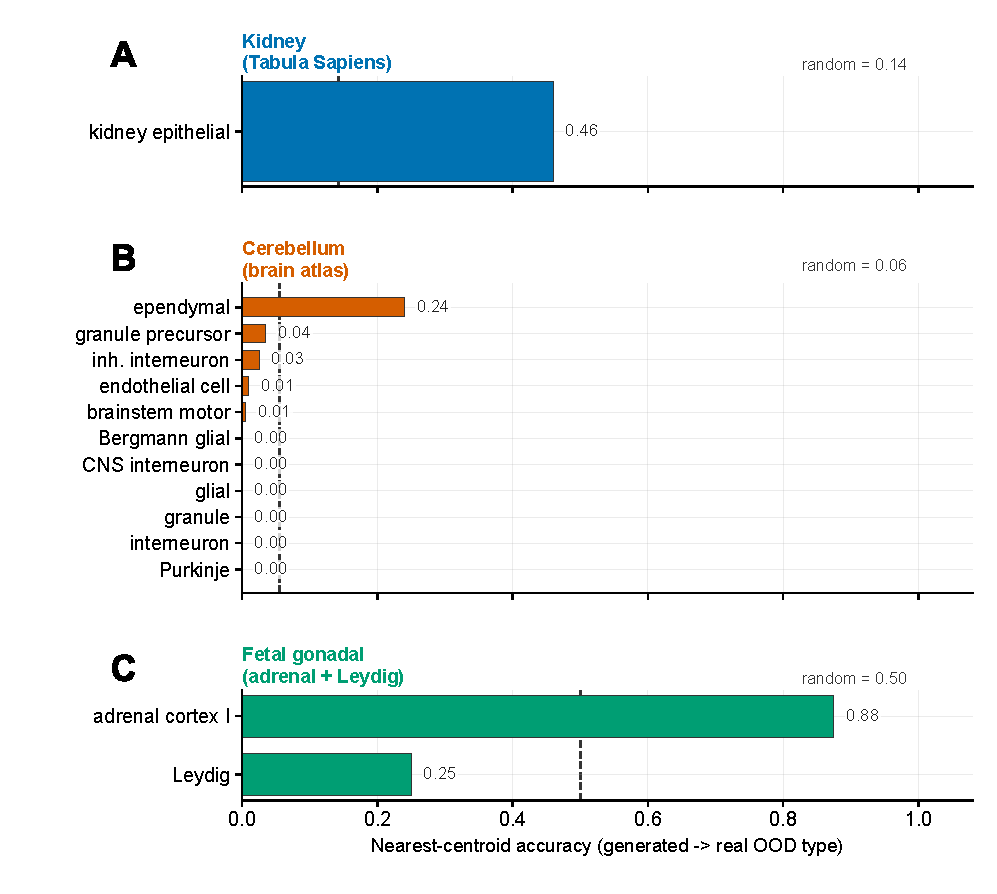
\includegraphics[width=0.95\textwidth]{Figure_09_strict_ood.pdf}
\caption{\textbf{Zero-shot strict-OOD generalization of CLOP-DiT by novel cell type.} Per-cell-type nearest-centroid accuracy for 14 cell types drawn from three strict-OOD tissues absent from the training corpus. Dashed lines mark random chance for the full OOD tissue vocabulary used by nearest-centroid scoring ($1/7$ kidney, $1/18$ cerebellum, $1/2$ fetal gonadal). Transfer is program-dependent: kidney epithelial reaches $0.460$ on the 7-way kidney baseline, and adrenal cortex type~I reaches $0.875$ on the 2-way fetal-gonadal baseline, consistent with epithelial/steroidogenic overlap with training tissues. Structurally distinct cerebellar neural programs remain at or below chance because the training corpus has no neural analog. A further sibling-collapse failure mode appears on the fetal gonadal sample, where Leydig-prompted outputs concentrate near the dominant adrenal centroid.\label{fig:strict-ood}}
\end{figure}

\begin{table}[!htbp]
\caption{Zero-shot strict-OOD generalization summary. ``Nearest-centroid accuracy'' is the fraction of generated cells whose closest real-cell-type centroid (within the same OOD tissue) equals the prompted target type. ``Random'' is $1/N_\text{types}$. ``FD'' is Gaussian Fr\'echet distance computed on the whitened 512-d space. See Figure~\ref{fig:strict-ood} for the per-cell-type breakdown.\label{tab:strict-ood}}
\centering
\small
\begin{tabular}{lrrrr}
\toprule
\textbf{Tissue (strict OOD)} & \textbf{Types} & \textbf{Nearest-acc} & \textbf{Random} & \textbf{FD} \\
\midrule
Kidney (Tabula Sapiens)         & 1  & 0.460 & 0.143 & 1.82 \\
Cerebellum (brain atlas)        & 11 & 0.029 & 0.056 & 1.62 \\
Testis / fetal gonadal          & 2  & 0.562 & 0.500 & 1.57 \\
\midrule
\textbf{Overall (mean)}         & --- & \textbf{0.350} & ---   & \textbf{1.67} \\
\bottomrule
\end{tabular}
\end{table}

The production CLOP-DiT \emph{partially} generalizes with sharp program-dependent variance. Two axes emerge clearly. First, structural-program transfer works, but with program-specific margins: kidney epithelial cell reaches $0.460$ against the 7-type kidney baseline (random $= 0.143$; about $3.2\times$), and adrenal cortex type~I reaches $0.875$ against the 2-type fetal-gonadal baseline (random $= 0.500$; about $1.75\times$), both despite the model having seen neither tissue during training. Steroidogenic and epithelial programs partially transfer through their shared transcriptional regulators (\emph{CYP17A1, STAR, NR5A1} on the steroidogenic side; \emph{CDH1, KRT18, EPCAM}-class on the epithelial side). Second, structurally-distinct programs do not transfer: cerebellar neurons are at or below random chance (Purkinje cells $0.00$; granule cells $0.00$; granule cell precursors $0.035$; inhibitory interneurons $0.025$; CNS interneurons $0.00$). The training corpus has no neural analog, so prompts describing GABAergic or glutamatergic cerebellar identities evoke a diffuse, type-agnostic conditional distribution. A complementary failure mode appears in the fetal gonadal sample, where Leydig-prompted outputs collapse toward the adrenal-cortex centroid ($0.25$ accuracy on a 2-way test versus $0.875$ for adrenal): sibling steroidogenic types are not resolved when one dominates the prompt space.

This is a boundary diagnostic rather than a binary pass/fail outcome. The zero-shot evaluation localizes the observed generalization boundary: the learned cross-type manifold extrapolates along familiar structural axes but not along unfamiliar ones. Combined with the upstream latent-compression diagnosis of Section~\ref{sec:rare-cell}, the heterogeneity-dominant failure axis of Section~\ref{sec:per-type}, and the partial-reversal Stage-1 ablation proxy of Section~\ref{sec:ablation}, the picture is internally consistent: under the tested configuration, the generator transfers best to novel contexts where training tissues cover the relevant expression program, while unsupported cell programs expose a training-coverage limit rather than evidence that architecture capacity is the limiting mechanism. Expanded training coverage to neural and gonadal tissues is an explicit next-step target.

%%%%%%%%%%%%%%%%%%%%%%%%%%%%%%%%%%%%%%%%%%
\FloatBarrier
\section{Discussion}\label{sec:discussion}

CLOP-DiT demonstrates that structured biological metadata can drive non-trivial single-cell latent generation, but the current model should be interpreted as an exploratory generator rather than a high-fidelity simulator. Its input is a practical structured scaffold of five biological fields, not unrestricted natural language, and its strongest evidence lies in latent-space type specificity and controllable steering rather than in indistinguishable expression-level realism.

\textbf{Unified mechanistic picture.} The major-revision analyses converge on a single diagnosis: CLOP-DiT's primary limitation is \emph{latent-stage under-dispersion of within-type heterogeneity}, not decoder collapse, not species imbalance, not data scarcity, and not a correctable-by-mixing downstream artefact. The decoder is expansive (rare-cell failure mechanism analysis and expression-scale Gaussian baselines in Section~\ref{sec:rare-cell}); species-stratified metrics are statistically equivalent (organism stratification, $p > 0.14$ on all headline metrics, Appendix~\ref{app:suppl-figs}); training-count abundance is a weak and wrong-signed predictor of per-type fidelity (abundance--fidelity analysis of Section~\ref{sec:per-type}, $\rho = +0.57$ vs.\ $\rho = -0.77$ for heterogeneity); classical augmentation mixing does not recover what the generator failed to produce (Section~\ref{sec:rare-cell}, flat or degrading F1 across all six strategies); and half of the remaining KNN errors are biologically graceful within-lineage confusions (KNN error taxonomy, Section~\ref{sec:per-type}, 49.2\% within-family). The improvement headroom is therefore concentrated at the generator: heterogeneity-preserving training objectives and latent-stage intervention.

\textbf{Variance and covariance deficits.} The main biological limitation is incomplete preservation of second-order structure. Even with the current DiT training objective, which augments flow matching with per-group variance matching ($\lambda_\text{var}=0.10$) and sliced covariance matching ($\lambda_\text{cov}=0.05$), within-type heterogeneity remains underrepresented. In-distribution variance trends are partly recovered ($r = 0.98$, Figure~\ref{fig:variance-deepdive}), but cross-dataset variance ratios, within-type gene--gene correlations, and rare-cell augmentation all indicate residual mean-collapse. The variance-matching pilot (Figure~\ref{fig:var-pilot}) reports per-type SWD, latent variance ratios, and per-dimension correlation ECDFs, while the gene--gene correlation panels (Figure~\ref{fig:gene-gene-corr}) show Mantel-correlation distributions and correlation-difference heatmaps for best- and worst-preserved types. In other words, group-aware latent regularization helps, but it is not sufficient on its own to recover realistic second-order biological structure.

\begin{figure}[!htbp]
\centering
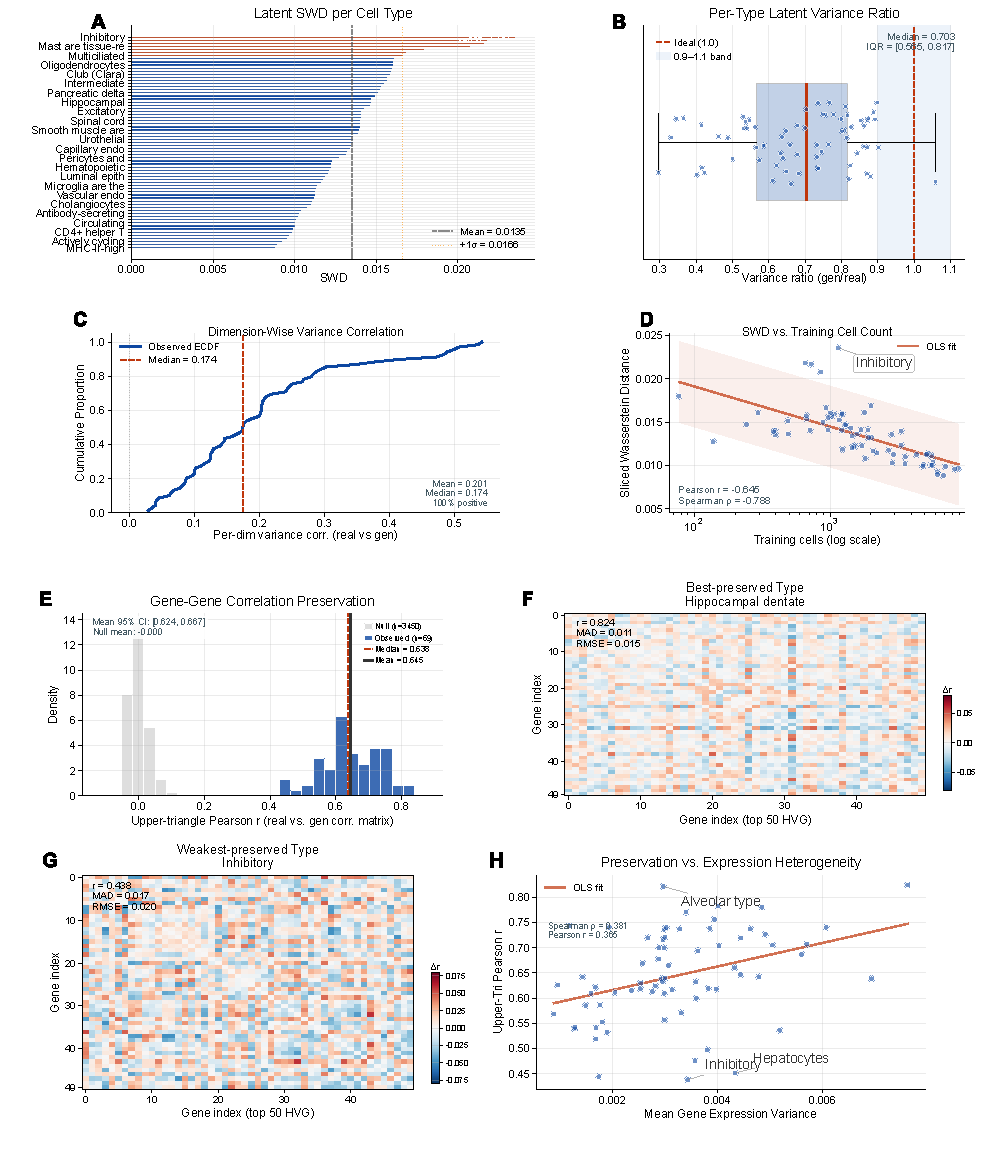
\includegraphics[width=0.95\textwidth]{Figure_10_variance_gene_correlation.pdf}
\caption{\textbf{Latent variance and gene--gene correlation analysis.} \emph{Variance matching} \textbf{A}~Per-cell-type sliced Wasserstein distance (SWD) between real and generated latent distributions. \textbf{B}~Per-type latent variance ratios (generated/real), summarized with the median and interquartile range relative to the ideal unity band. \textbf{C}~Per-dimension variance-correlation ECDF, showing that most dimensions remain positively correlated but only weakly structured. \textbf{D}~SWD versus training cell count with Pearson and Spearman trend summaries. \emph{Gene--gene correlation} \textbf{E}~Distribution of per-type Mantel correlations with a permuted-null baseline overlay and bootstrap confidence interval on the mean preserved correlation. \textbf{F--G}~Correlation-difference heatmaps for best- and worst-preserved cell types. \textbf{H}~Mantel $r$ versus mean gene expression variance per type, showing only a weak dependence of preservation on intrinsic heterogeneity.\label{fig:var-pilot}\label{fig:gene-gene-corr}}
\end{figure}

\textbf{Extended validation.} Five additional experiments characterize the model beyond the core latent metrics; full figures are provided in Appendix~\ref{app:suppl-figs}. Cross-dataset validation across five tissues confirms near-perfect mean reconstruction after shared decoder reconstruction but near-zero variance correlation, underscoring that decoder consistency is not the same as transcriptomic fidelity. Expanded differential-expression analyses, OOD prompt tests, marker-completeness scores, and rare-cell augmentation collectively reinforce the same message: the model captures coarse biological identity better than within-type heterogeneity. The OOD free-form prompts (Figure~\ref{fig:ood-showcase}, panel C), cross-dataset mean correlation (Figure~\ref{fig:cross-dataset}, panel D), expanded DE concordance (Figure~\ref{fig:expanded-de}, panel E), OOD marker-hit rates (Figure~\ref{fig:ood-robustness}, panel F), marker recall@$K$ curves (Figure~\ref{fig:marker-completeness}, panel G), and six-axis validation radar (Figure~\ref{fig:validation-summary}, panel H) are rendered in Appendix~\ref{app:suppl-figs}, together with per-cell-type pseudobulk correlation (Figure~\ref{fig:pseudobulk}, panels A--B) and failure-mode stratification (Figure~\ref{fig:failure-analysis}, panels C--E).

\textbf{Ablation, reproducibility, and decoder analysis.} The CLOP ablation heatmap (Figure~\ref{fig:ablation-heatmap}, panel A) consolidates 15 experiments and confirms that cohesion and noise regularization materially affect alignment quality (Table~\ref{tab:ablation}). Multi-seed validation (Figure~\ref{fig:multi-seed}, panel B) shows stable steering ($\sigma = 0.009$) and diversity ($\sigma \leq 0.016$) across three independent runs (Table~\ref{tab:multi-seed}). Decoder ablations comparing frozen scGPT, LoRA-adapted, and MLP decoders (Figure~\ref{fig:decoder-ablation}, panel L) produce broadly similar expression profiles, and embedding-level augmentation $\Delta$F1 at 1$\times$--10$\times$ ratios (Figure~\ref{fig:embedding-augmentation}, panel K) remains flat, suggesting that the main bottleneck lies upstream of the decoder: in the latent generator and the geometry of the aligned embedding space.

\textbf{Benchmarking and operating regimes.} On the primary common-metrics-only comparison, the Gaussian baseline outperforms CLOP-DiT, underscoring that mean-matching remains competitive when evaluation is restricted to global distributional similarity. The distinctive value of CLOP-DiT lies instead in conditional controllability: CFG = 2.0 with Euler sampling emphasizes type fidelity, whereas CFG = 1.0 with Midpoint sampling preserves substantially more diversity. Neither regime closes the gap to real data (KNN 36.9\%, discriminator AUC 0.656), but together they provide an interpretable operating envelope rather than a single opaque optimum.

\textbf{Limitations and scope.} The 36.9\% KNN accuracy still implies substantial label uncertainty; the high-fidelity regime (DivR = 0.513) remains centroid-biased; and the rare-cell augmentation experiment was negative at both expression and embedding levels. All results are restricted to human and mouse cancer/developmental datasets. Species-stratified analysis (18 human-only, 8 mouse-only, 43 dual-organism types) shows no statistically significant bias attributable to organism at the type level ($p > 0.14$ on all headline metrics), but the evaluation remains in-distribution on the same cell-type vocabulary.

\textbf{Strict out-of-distribution generalization.} Section~\ref{sec:strict-ood} reports a zero-shot strict-OOD evaluation on kidney, cerebellum, and fetal gonadal tissue (Table~\ref{tab:strict-ood}). The production CLOP-DiT partially generalizes to novel cell types with sharp program-dependent variance: kidney epithelial reaches $0.460$ on a 7-type random baseline of $0.143$, and adrenal cortex type~I reaches $0.875$ on a 2-type random baseline of $0.500$, but structurally-distinct novel neural types remain at or below random (Purkinje cells $= 0.00$, cerebellar interneurons $= 0.00$). We interpret this as a boundary test: the learned cross-type manifold extrapolates along familiar structural axes (epithelial, steroidogenic) but not along unfamiliar ones (GABAergic cerebellar neurons). Combined with the upstream latent-compression diagnosis (A5) and the scGPT-specific compression result (Section~\ref{sec:decoding} decoder analysis), the current evidence points to training-corpus coverage at the cell-program level as the practical limiting factor under this configuration, rather than proving an intrinsic architecture or decoder-capacity ceiling. Expanded training coverage to neural and gonadal tissues is the targeted next step, and we treat full strict-OOD \emph{retraining} (as opposed to today's zero-shot evaluation) as an explicit future-work item.

\textbf{Where the bottleneck lives (encoder-side localization).} Three independent input-side levers all fail to move within-type latent variance in the scGPT embedding space. (i)~Relaxing the per-dataset cell cap from 3{,}000 to 10{,}000 cells ($3.12\times$ more input cells, with a fixed \texttt{sc.pp.subsample} seed on both sides) leaves the median per-dataset total-variance ratio at 1.008 (IQR [0.984, 1.035]) and the median within-cluster variance ratio at 0.976 across 475 matched (dataset, cell-type) pairs. (ii)~Sweeping the HVG count from 500 to 8{,}000 genes produces less than a $5\%$ change in latent within-cluster variance once the HVG count exceeds 2{,}000; the curve saturates rather than scaling with gene budget. (iii)~A direct raw-vs-latent compression diagnostic shows that the encoder compresses within-type L2 distance by a median factor of $6\times$ (ratio 0.168, IQR [0.132, 0.214]) while shrinking between-type centroid distance only $3.7\times$ (ratio 0.274). These three converging null results indicate that, under the frozen scGPT encoder used here, within-type heterogeneity is constrained primarily by representation geometry rather than by the tested data-scaling or preprocessing choices. A matched-dimensionality encoder comparison on eight representative datasets (Table~\ref{tab:encoder-comparison}) supports this as an scGPT-specific compression pattern rather than a generic consequence of using a 512-dimensional space. In the same 512-d space, PCA preserves within-type distance almost intact (median ratio $0.90$), whereas scGPT-human compresses it $\sim 7\times$ (median ratio $0.14$) and scGPT-pancancer compresses it $\sim 15\times$ (median ratio $0.07$). Tightness ratios remain comparable across scGPT variants ($\sim 0.65$), indicating that the transformer constructs good between-type structure while disproportionately discarding within-type fine structure. This localizes a major fraction of the residual generation gap upstream of the diffusion generator---in the cell encoder's learned representation geometry under the tested encoders---and motivates a heterogeneity-preserving encoder objective (or an alternative encoder) as the next targeted step beyond prompt-side or decoder-side interventions.

\begin{table}[!htbp]
\caption{Matched-dimensionality encoder comparison on eight representative datasets (same within/between L2 tightness metric as the encoder-bottleneck diagnostic). Within-L2 ratio is encoder-space within-type distance divided by raw-space within-type distance (lower = more within-type compression); tightness ratio is the encoder-space within/between ratio divided by its raw-space counterpart (lower = clusters more separable relative to raw). All three encoders map to a 512-dimensional space. PCA is fitted per-dataset. scGPT variants are frozen pre-trained checkpoints.\label{tab:encoder-comparison}}
\centering
\begingroup
\footnotesize
\setlength{\tabcolsep}{4pt}
\begin{tabular}{@{}lccc@{}}
\toprule
\textbf{Encoder} & \textbf{Within-L2 median} & \textbf{Within-L2 IQR} & \textbf{Tightness median} \\
\midrule
PCA (linear, 512-d) & 0.899 & [0.890, 0.922] & 0.900 \\
scGPT-human (33M cells) & 0.144 & [0.121, 0.181] & 0.647 \\
scGPT-pancancer (5.7M cells) & 0.066 & [0.051, 0.086] & 0.670 \\
\bottomrule
\end{tabular}
\endgroup
\end{table}

Moreover, because the decoder is frozen, expression-level agreement should be interpreted as a property of the full pipeline rather than as evidence that the model faithfully reproduces raw counts.

\textbf{Modular architecture as a path forward.} CLOP-DiT's three-stage design still offers a practical route for targeted improvement. Future work can strengthen the existing variance/covariance objectives, fine-tune or adapt the decoder, and enrich the prompt encoder without rewriting the entire pipeline. This composability distinguishes CLOP-DiT from fully joint training approaches~\cite{ref-scdesign3} and makes it a useful scaffold for iterative methodological improvement.

%%%%%%%%%%%%%%%%%%%%%%%%%%%%%%%%%%%%%%%%%%
\section{Conclusions}\label{sec:conclusions}

We introduced CLOP-DiT, a three-stage framework for generating single-cell latents from structured metadata. By aligning structured captions and cell embeddings, sampling new latents with a condition-aware Diffusion Transformer, and decoding them through scGPT, the pipeline establishes that biologically meaningful text-guided generation is feasible in principle. Across 69 deduplicated cell types from 80 GEO datasets, the model delivers above-chance type specificity, reproducible fidelity--diversity operating regimes, and causal evidence that prompt fields---especially marker genes---steer generation.

\textbf{Scope of claims.} The study also makes its current boundary conditions explicit. All results are limited to in-distribution human and mouse cancer/developmental datasets, latent-space metrics remain more trustworthy than decoder-level expression agreement, and within-type heterogeneity is still under-preserved despite variance- and covariance-aware regularization. CLOP-DiT should therefore be viewed as a modular proof of concept rather than as a finished simulator for downstream biological decision-making.

\textbf{Future directions.} The modular architecture nevertheless offers several concrete next steps: (i)~strengthening the existing variance- and covariance-aware training objectives; (ii)~decoder fine-tuning via adapters such as LoRA~\cite{ref-scgpt}; (iii)~adaptive ODE sampling for improved distributional fidelity; (iv)~more rigorous out-of-distribution evaluation on unseen cell types and organisms; and (v)~direct benchmarking against CellWhisperer~\cite{ref-cellwhisperer} and scDesign3~\cite{ref-scdesign3} under harmonized evaluation protocols.

%%%%%%%%%%%%%%%%%%%%%%%%%%%%%%%%%%%%%%%%%%

%%%%%%%%%%%%%%%%%%%%%%%%%%%%%%%%%%%%%%%%%%
%% optional
%% No separate supplementary files are provided; all supplementary tables
%% (Tables S1--S5) are included in Appendix~D of this article.

% Only for journal Methods and Protocols:
% If you wish to submit a video article, please do so with any other supplementary material.
% \supplementary{The following supporting information can be downloaded at: \linksupplementary{s1}, Figure S1: title; Table S1: title; Video S1: title. A supporting video article is available at doi: link.}

% Only used for preprtints:
% \supplementary{The following supporting information can be downloaded at the website of this paper posted on \href{https://www.preprints.org/}{Preprints.org}.}

% Only for journal Hardware:
% If you wish to submit a video article, please do so with any other supplementary material.
% \supplementary{The following supporting information can be downloaded at: \linksupplementary{s1}, Figure S1: title; Table S1: title; Video S1: title.\vspace{6pt}\\
%\begin{tabularx}{\textwidth}{lll}
%\toprule
%\textbf{Name} & \textbf{Type} & \textbf{Description} \\
%\midrule
%S1 & Python script (.py) & Script of python source code used in XX \\
%S2 & Text (.txt) & Script of modelling code used to make Figure X \\
%S3 & Text (.txt) & Raw data from experiment X \\
%S4 & Video (.mp4) & Video demonstrating the hardware in use \\
%... & ... & ... \\
%\bottomrule
%\end{tabularx}
%}

%%%%%%%%%%%%%%%%%%%%%%%%%%%%%%%%%%%%%%%%%%
\authorcontributions{Z.F.: conceptualization, methodology, software, validation, formal analysis, investigation, resources, data curation, writing---original draft preparation, visualization, project administration. Y.L., J.W., and S.W.: writing---review and editing, supervision, and funding acquisition. All authors have read and agreed to the published version of the manuscript.}

\funding{This work was supported by the National Key Research and Development Program of China (Grant No.~2024YFA1107101), the Ministry of Science and Technology of the People\textquotesingle s Republic of China, and the National Key Laboratory of Trauma and Chemical Poisoning (Grant No.~2024K004).}

\institutionalreview{Ethical review and approval were waived for this study, as only publicly available, de-identified data from the Gene Expression Omnibus (GEO) were analyzed; all datasets were deposited by their original investigators under institutional ethical approvals as required by GEO submission policy. No new human subjects research, animal experiments, or clinical interventions were conducted.}

\informedconsent{Not applicable.}

\dataavailability{The training and validation data were curated from publicly available GEO datasets; a full list of GEO accession identifiers is provided in Table~\ref{tab:s1_datasets} (Appendix~\ref{app:suppl-tables}), and the held-out validation study identifiers are in Table~\ref{tab:s2_validation}. Source code, trained model checkpoints (CLOP aligner and DiT generator), configuration files, environment specifications (Python~3.10, PyTorch~2.1, CUDA~12.0, scGPT~v0.2.1, Transformers~4.36), multi-seed validation data, independent marker gene validation data (PanglaoDB and CellMarker~2.0 cross-references), external marker ablation analysis, and one-command figure reproduction instructions are publicly available on GitHub~\cite{ref-clop-dit} and will be archived on Zenodo upon acceptance of this manuscript. All figures use colormaps designed for accessibility under common forms of color vision deficiency (deuteranopia, protanopia); critical distinctions additionally use shape or pattern encoding.}

%\durcstatement{Current research is limited to the [please insert a specific academic field, e.g., XXX], which is beneficial [share benefits and/or primary use] and does not pose a threat to public health or national security. Authors acknowledge the dual-use potential of the research involving xxx and confirm that all necessary precautions have been taken to prevent potential misuse. As an ethical responsibility, authors strictly adhere to relevant national and international laws about DURC. Authors advocate for responsible deployment, ethical considerations, regulatory compliance, and transparent reporting to mitigate misuse risks and foster beneficial outcomes.}

% Only for journal Nursing Reports
%\publicinvolvement{Please describe how the public (patients, consumers, carers) were involved in the research. Consider reporting against the GRIPP2 (Guidance for Reporting Involvement of Patients and the Public) checklist. If the public were not involved in any aspect of the research add: ``No public involvement in any aspect of this research''.}
%
%% Only for journal Nursing Reports
%\guidelinesstandards{Please add a statement indicating which reporting guideline was used when drafting the report. For example, ``This manuscript was drafted against the XXX (the full name of reporting guidelines and citation) for XXX (type of research) research''. A complete list of reporting guidelines can be accessed via the equator network: \url{https://www.equator-network.org/}.}
%
%% Only for journal Nursing Reports

\acknowledgments{The author acknowledges the developers and communities behind scGPT, BiomedBERT, and the Gene Expression Omnibus (GEO) for providing open-access tools and datasets that made this work possible.}

\conflictsofinterest{The author declares no conflicts of interest.}

%%%%%%%%%%%%%%%%%%%%%%%%%%%%%%%%%%%%%%%%%%
%% Optional

%% Only for journal Encyclopedia
%\entrylink{The Link to this entry published on the encyclopedia platform.}

\abbreviations{Abbreviations}{
The following abbreviations are used in this manuscript:\\\noindent
\begin{tabular}{@{}ll}
AdaLN & Adaptive Layer Normalization\\
CFG & Classifier-free guidance\\
CLOP & Contrastive Language-Omics Pretraining\\
DE & Differential expression\\
DiT & Diffusion Transformer\\
DivR & Diversity Ratio\\
EMA & Exponential Moving Average\\
FD & Fr\'{e}chet Distance\\
GEO & Gene Expression Omnibus\\
KNN & $k$-Nearest Neighbor\\
LinAcc & Linear Classifier Accuracy\\
logFC & Log Fold Change\\
LoRA & Low-Rank Adaptation\\
ODE & Ordinary Differential Equation\\
OOD & Out-of-Distribution\\
scGPT & Single-cell Generative Pre-trained Transformer\\
scRNA-seq & Single-cell RNA sequencing\\
SigLIP & Sigmoid Loss for Language-Image Pre-training\\
ZCA & Zero-phase Component Analysis
\end{tabular}
}

%%%%%%%%%%%%%%%%%%%%%%%%%%%%%%%%%%%%%%%%%%
%% Optional
\appendixtitles{yes}
\FloatBarrier
\clearpage
\appendixstart
\FloatBarrier
\appendix
% Appendix-local figure/table renumbering: figures become A1, A2, ...;
% tables become A1, A2, ... (same-letter namespace as figures — use \ref
% with a fig: or tab: prefix to disambiguate in cross-references).
\renewcommand{\thefigure}{A\arabic{figure}}
\setcounter{figure}{0}
\renewcommand{\thetable}{A\arabic{table}}
\setcounter{table}{0}
% Tighten caption spacing for the appendix: less whitespace between image
% and its caption block so supplementary-figure captions sit close under
% the panel content instead of stranded at the bottom of the page.
\setlength{\abovecaptionskip}{4pt}
\setlength{\belowcaptionskip}{0pt}
\section[\appendixname~\thesection]{Supplementary Material}\label{app:suppl-tables}\label{app:hyperparams}

\begin{table}[!htbp]
\caption{Architecture specifications.\label{tab:architecture}}
\begin{tabularx}{\textwidth}{lCC}
\toprule
\textbf{Component} & \textbf{Architecture} & \textbf{Parameters} \\
\midrule
BiomedBERT-large (frozen) & Transformer encoder  & 340M \\
CLOP text projector       & MLP [1024$\to$1024$\to$1024$\to$512] & 1.58M \\
CLOP cell projector       & MLP [512$\to$512$\to$512$\to$512]    & 1.44M \\
DiT1D                     & 8$\times$ AdaLN-Zero blocks, 8 heads & 22.10M \\
scGPT encoder (frozen)    & Transformer                          & $\sim$51M \\
scGPT decoder (frozen)    & Gene token prediction head           & included \\
\bottomrule
\end{tabularx}
\end{table}

\begin{table}[!htbp]
\caption{CFG scale sweep (10-step Euler, 69 eval groups). Values are computed on a different subsample (69 groups $\times$ 200 cells) than the primary operating-point results in Table~\ref{tab:core-results} (69 types $\times$ 200 cells with different random seeds), which accounts for minor numerical differences.\label{tab:cfg-sweep}}
\centering
\begin{tabular}{lrrrr}
\toprule
\textbf{CFG} & \textbf{KNN-1} & \textbf{Steering} & \textbf{DivR} & \textbf{KNN/Random} \\
\midrule
0.5 & 0.147 & 0.788 & 1.13 & 15$\times$ \\
1.0 & 0.348 & 0.796 & 0.76 & 35$\times$ \\
1.5 & 0.396 & 0.798 & 0.60 & 40$\times$ \\
2.0 & 0.407 & 0.806 & 0.53 & 41$\times$ \\
2.5 & 0.408 & 0.804 & 0.49 & 41$\times$ \\
3.0 & 0.410 & 0.802 & 0.48 & 41$\times$ \\
4.0 & 0.402 & 0.804 & 0.50 & 40$\times$ \\
5.0 & 0.380 & 0.798 & 0.55 & 38$\times$ \\
\bottomrule
\end{tabular}
\end{table}

\begin{table}[!htbp]
\caption{Training hyperparameters for both CLOP alignment and DiT flow-matching stages.\label{tab:hyperparams}}
\begin{tabularx}{\textwidth}{lCC}
\toprule
\textbf{Hyperparameter} & \textbf{CLOP} & \textbf{DiT} \\
\midrule
Optimizer         & AdamW              & AdamW ($\beta_1{=}0.9, \beta_2{=}0.999$) \\
Learning rate     & $5 \times 10^{-4}$ & $2 \times 10^{-4}$ \\
Weight decay      & 0.06               & 0.01 \\
Batch size        & 1024               & 1024 \\
Epochs            & 100                & 300 \\
Warmup epochs     & 5                  & 5 \\
LR schedule       & Cosine with warmup & Cosine with warmup \\
Gradient clipping  & 1.0               & 1.0 \\
Mixed precision   & FP16 (AMP)         & FP16 (AMP) \\
Dropout           & 0.2                & Proj: 0.1, Attn: 0.0 \\
EMA decay         & ---                & 0.9999 \\
Temperature       & 14.0 (fixed; see Section~\ref{sec:clop})       & --- \\
Loss              & PrototypeSigLIP    & Flow matching + variance/covariance regularization \\
Cohesion weight   & 0.15               & --- \\
Variance loss wt. & ---                & 0.10 \\
Covariance loss wt. & ---              & 0.05 \\
Label smoothing   & 0.1                & --- \\
CFG drop prob     & ---                & 0.15 \\
Time sampling     & ---                & Logit-normal ($\mu{=}0, \sigma{=}1$) \\
\bottomrule
\end{tabularx}
\end{table}

% Table S1: All 80 GEO Dataset Identifiers (data from Table_S1_GEO_Accessions.tsv)
{\footnotesize
\renewcommand{\arraystretch}{0.9}
\begin{longtable}{rllp{4.2cm}rr}
\caption{All 80 GEO datasets used in CLOP-DiT training and validation. Datasets were preprocessed to 2{,}000 highly variable genes per dataset. Split: Train or held-out Validation (study-level, seed 42). Hs: \textit{Homo sapiens}; Mm: \textit{Mus musculus}.\label{tab:s1_datasets}} \\
\toprule
\# & Accession & Organism & Description & $n_{\text{cells}}$ & Split \\
\midrule
\endfirsthead
\toprule
\# & Accession & Organism & Description & $n_{\text{cells}}$ & Split \\
\midrule
\endhead
\midrule
\multicolumn{6}{r}{\textit{Continued on next page}} \\
\endfoot
\bottomrule
\endlastfoot
  1 & GSE103867 & Hs & scRNA-seq (GEO-DataHub) & 2,787 & Val \\
  2 & GSE110686 & Hs & scRNA-seq (GEO-DataHub) & 2,992 & Train \\
  3 & GSE115571 & Mm & Mouse cells, LPS stimulation & 442 & Train \\
  4 & GSE117988 & Hs & PBMCs, Merkel cell carcinoma & 2,638 & Train \\
  5 & GSE117988 & Hs & Merkel cell carcinoma tumor & 2,990 & Train \\
  6 & GSE120505 & Hs & Aged blood cells & 3,000 & Train \\
  7 & GSE123813 & Hs & Basal cell carcinoma skin & 3,000 & Train \\
  8 & GSE123813 & Hs & Cutaneous squamous cell carcinoma & 3,000 & Train \\
  9 & GSE123902 & Hs & Lung adenocarcinoma & 2,753 & Train \\
  10 & GSE124310 & Hs & Multiple myeloma bone marrow & 2,833 & Train \\
  11 & GSE130148 & Hs & Fetal lung development & 3,000 & Train \\
  12 & GSE132509 & Hs & Pediatric ALL bone marrow & 2,984 & Train \\
  13 & GSE138709 & Hs & Intrahepatic cholangiocarcinoma & 2,891 & Train \\
  14 & GSE142653 & Hs & Pituitary gland development & 2,885 & Train \\
  15 & GSE143423 & Hs & Leptomeningeal brain metastasis & 3,000 & Train \\
  16 & GSE143423 & Hs & Triple-neg.\ breast cancer brain met. & 2,332 & Train \\
  17 & GSE145929 & Mm & Adult mouse prostate & 2,830 & Train \\
  18 & GSE145929 & Mm & Adult mouse urethra & 2,745 & Train \\
  19 & GSE148218 & Hs & Bone marrow, ALL & 2,807 & Train \\
  20 & GSE149655 & Hs & Early-stage lung adenocarcinoma & 2,087 & Train \\
  21 & GSE155109 & Hs & Endothelial cells, breast cancer & 3,000 & Train \\
  22 & GSE155109 & Hs & Stromal cells, breast cancer & 3,000 & Train \\
  23 & GSE163558 & Hs & Stomach cancer & 2,467 & Train \\
  24 & GSE165784 & Hs & Retina development & 2,622 & Train \\
  25 & GSE165844 & Mm & LSK hematopoietic progenitors & 2,881 & Train \\
  26 & GSE167597 & Mm & Spinal cord development & 3,000 & Val \\
  27 & GSE168181 & Hs & Breast cancer tissue & 2,863 & Train \\
  28 & GSE175975 & Hs & scRNA-seq (GEO-DataHub) & 2,728 & Train \\
  29 & GSE183904 & Hs & Gastric cancer & 3,000 & Val \\
  30 & GSE189070 & Mm & Astrocytes, spinal cord injury & 2,960 & Train \\
  31 & GSE189357 & Hs & Lung adenocarcinoma & 2,886 & Train \\
  32 & GSE192857 & Hs & hESC differentiation time-series & 2,696 & Train \\
  33 & GSE212502 & Hs & Forebrain organoids & 3,000 & Train \\
  34 & GSE213740 & Hs & Ascending aortic wall dissection & 2,704 & Val \\
  35 & GSE220913 & Hs & HL-60 cell lines, CFTR & 2,972 & Train \\
  36 & GSE222002 & Hs & T cells from cancer & 2,962 & Train \\
  37 & GSE222369 & Hs & NK cells, lymphoma & 2,778 & Train \\
  38 & GSE225600 & Hs & Breast cancer tumor & 2,333 & Train \\
  39 & GSE225857 & Hs & Colorectal cancer liver metastases & 2,986 & Train \\
  40 & GSE226131 & Mm & Aged hematopoietic stem cells & 2,608 & Train \\
  41 & GSE226762 & Hs & scRNA-seq (GEO-DataHub) & 830 & Val \\
  42 & GSE227644 & Hs & scRNA-seq (GEO-DataHub) & 3,000 & Train \\
  43 & GSE227719 & Mm & KrasG12D/P53 lung organoids & 2,990 & Train \\
  44 & GSE228499 & Hs & Breast cancer & 2,448 & Train \\
  45 & GSE235787 & Hs & B cells, ALL & 2,798 & Train \\
  46 & GSE236565 & Mm & Splenic CD4+ T cells & 2,556 & Train \\
  47 & GSE248214 & Hs & scRNA-seq (GEO-DataHub) & 2,998 & Train \\
  48 & GSE253355 & Hs & Bone marrow niche & 2,835 & Train \\
  49 & GSE262288 & Hs & Metastatic breast cancer & 2,321 & Train \\
  50 & GSE272187 & Hs & scRNA-seq (GEO-DataHub) & 2,639 & Train \\
  51 & GSE275119 & Mm & Dental tissue development & 2,963 & Train \\
  52 & GSE277740 & Mm & Thalamus, SBS vs DNBSEQ & 2,644 & Val \\
  53 & GSE279781 & Hs & scRNA-seq (GEO-DataHub) & 2,654 & Train \\
  54 & GSE280847 & Mm & CD45+ leukocytes, MC38 tumor & 2,864 & Train \\
  55 & GSE283205 & Hs & Hepatoblastoma tumor tissue & 2,994 & Train \\
  56 & GSE283397 & Hs & CD8+ T cells, CLL & 2,856 & Train \\
  57 & GSE288211 & Mm & Pancreatic islets, Zzef1 KO & 2,724 & Train \\
  58 & GSE289611 & Hs & Pulmonary pleomorphic carcinoma & 2,983 & Train \\
  59 & GSE291166 & Mm & Mesenteric lymph node & 2,901 & Train \\
  60 & GSE299623 & Hs & scRNA-seq (GEO-DataHub) & 2,991 & Train \\
  61 & GSE300862 & Mm & Kras/Trp53 lung adenocarcinoma & 2,716 & Val \\
  62 & GSE302433 & Mm & B16F10 melanoma, ZDHHC13 & 2,953 & Val \\
  63 & GSE303309 & Mm & Brain CD45+ immune cells, AD & 2,999 & Train \\
  64 & GSE306567 & Mm & ESCs and neural progenitors & 2,454 & Train \\
  65 & GSE306676 & Mm & Spinal cord, SOD1-G93A ALS & 2,959 & Train \\
  66 & GSE307261 & Hs & B and T cells, melanoma & 2,921 & Train \\
  67 & GSE307774 & Mm & Colorectal tumors, Kras/Braf & 2,505 & Train \\
  68 & GSE308428 & Mm & Hippocampal microglia, ASD & 2,991 & Train \\
  69 & GSE309368 & Hs & Myeloid cells, oral SCC & 1,361 & Train \\
  70 & GSE315628 & Mm & scRNA-seq (GEO-DataHub) & 2,895 & Train \\
  71 & GSE318353 & Hs & scRNA-seq (GEO-DataHub) & 2,964 & Train \\
  72 & GSE98638  & Hs & HCC T cell landscape & 3,000 & Train \\
  73 & GSE120446 & Hs & Bone marrow, hematopoietic dev. & 2,890 & Train \\
  74 & GSE104323 & Mm & Dentate gyrus, brain development & 3,000 & Train \\
  75 & GSE75748  & Hs & Endoderm differentiation & 2,531 & Train \\
  76 & GSE144024 & Hs & Human embryonic stem cells & 3,000 & Train \\
  77 & GSE72857  & Mm & Hematopoiesis & 3,000 & Train \\
  78 & GSE226824 & Hs & IFN-treated HSPCs & 2,739 & Train \\
  79 & GSE141259 & Mm & Lung development & 3,000 & Train \\
  80 & GSE139369 & Hs & Hematopoiesis (Setty et al.) & 2,995 & Train \\
\midrule
  & \textbf{Total} & & & \textbf{220,304} & \\
\end{longtable}
}% end footnotesize for Table S1

% Table S2: 8 Held-out Validation Datasets (data from Table_S2_Validation_Datasets.tsv)
\begin{table}[!htbp]
\centering
\caption{The 8 held-out validation datasets (study-level split, seed 42, val\_split = 0.1). No cells from these studies were seen during CLOP or DiT training. Hs: \textit{Homo sapiens}; Mm: \textit{Mus musculus}.\label{tab:s2_validation}}
\begin{tabular}{rllp{4.5cm}r}
\toprule
\# & Accession & Organism & Description & $n_{\text{cells}}$ \\
\midrule
  1 & GSE103867 & Hs & scRNA-seq (GEO-DataHub) & 2,787 \\
  2 & GSE167597 & Mm & Mouse spinal cord development & 3,000 \\
  3 & GSE183904 & Hs & Gastric cancer & 3,000 \\
  4 & GSE213740 & Hs & Ascending aortic wall dissection & 2,704 \\
  5 & GSE226762 & Hs & scRNA-seq (GEO-DataHub) & 830 \\
  6 & GSE277740 & Mm & Thalamus, SBS vs DNBSEQ & 2,644 \\
  7 & GSE300862 & Mm & Kras/Trp53 lung adenocarcinoma & 2,716 \\
  8 & GSE302433 & Mm & B16F10 melanoma, ZDHHC13 & 2,953 \\
\midrule
  & \textbf{Total} & & \textbf{20,634} \\
\bottomrule
\end{tabular}
\end{table}

% Table S3: Full CFG Scale / Solver / Steps Sweep Results
{\footnotesize
\renewcommand{\arraystretch}{0.9}
\begin{longtable}{lllrrrrrr}
\caption{Full CFG scale sweep. 200 cells generated per group (69 groups). KNN: type-identity accuracy; Steer.: alignment; DivR: diversity ratio (1.0 = ideal); LinAcc: linear classifier accuracy; FD: Fr\'{e}chet distance.\label{tab:s3_cfg_sweep}} \\
\toprule
CFG & Solver & Steps & KNN-1 & KNN-5 & Steer. & DivR & LinAcc & FD \\
\midrule
\endfirsthead
\toprule
CFG & Solver & Steps & KNN-1 & KNN-5 & Steer. & DivR & LinAcc & FD \\
\midrule
\endhead
\midrule
\multicolumn{9}{r}{\textit{Continued on next page}} \\
\endfoot
\bottomrule
\endlastfoot
\multicolumn{9}{l}{\textit{Primary configurations (Table~\ref{tab:core-results})}} \\
\midrule
  3.0 & Euler & 10 & 0.367 & 0.554 & 0.802 & 0.473 & 0.508 & 3.46 \\
  2.0 & Euler & 10 & 0.369 & 0.553 & 0.810 & 0.513 & 0.511 & 3.17 \\
  1.0 & Euler & 10 & 0.313 & 0.483 & 0.810 & 0.745 & 0.390 & 2.84 \\
  0.0 & Euler & 10 & 0.010 & 0.051 & 0.475 & 1.833 & 0.010 & 0.58 \\
  3.0 & Midpoint & 10 & 0.340 & 0.528 & 0.792 & 0.628 & 0.477 & 3.38 \\
  2.0 & Midpoint & 10 & 0.340 & 0.525 & 0.800 & 0.686 & 0.475 & 3.13 \\
  1.0 & Midpoint & 10 & 0.288 & 0.461 & 0.807 & 0.929 & 0.357 & 2.64 \\
  3.0 & Euler & 50 & 0.348 & 0.545 & 0.795 & 0.622 & 0.489 & 3.33 \\
  1.0 & Euler & 50 & 0.293 & 0.466 & 0.807 & 0.919 & 0.365 & 2.65 \\
  --- & Gaussian & --- & 0.011 & 0.048 & 0.466 & 2.277 & 0.009 & 0.03 \\
\midrule
\multicolumn{9}{l}{\textit{Fine-grained CFG sweep (Euler solver)}} \\
\midrule
  0.5 & Euler & 10 & 0.147 & 0.284 & 0.788 & 1.129 & --- & 2.33 \\
  1.0 & Euler & 10 & 0.348 & 0.515 & 0.796 & 0.757 & --- & 2.94 \\
  1.5 & Euler & 10 & 0.396 & 0.553 & 0.798 & 0.600 & --- & 3.36 \\
  2.0 & Euler & 10 & 0.407 & 0.580 & 0.806 & 0.526 & --- & 3.54 \\
  2.5 & Euler & 10 & 0.408 & 0.590 & 0.804 & 0.493 & --- & 3.70 \\
  3.0 & Euler & 10 & 0.410 & 0.592 & 0.802 & 0.484 & --- & 3.80 \\
  4.0 & Euler & 10 & 0.402 & 0.586 & 0.804 & 0.502 & --- & 4.01 \\
  5.0 & Euler & 10 & 0.380 & 0.576 & 0.798 & 0.548 & --- & 4.34 \\
  0.5 & Euler & 20 & 0.137 & 0.269 & 0.788 & 1.230 & --- & 2.07 \\
  1.0 & Euler & 20 & 0.334 & 0.504 & 0.794 & 0.842 & --- & 2.83 \\
  1.5 & Euler & 20 & 0.380 & 0.545 & 0.798 & 0.679 & --- & 3.19 \\
  2.0 & Euler & 20 & 0.391 & 0.569 & 0.798 & 0.600 & --- & 3.43 \\
  2.5 & Euler & 20 & 0.394 & 0.578 & 0.800 & 0.559 & --- & 3.66 \\
  3.0 & Euler & 20 & 0.398 & 0.582 & 0.800 & 0.540 & --- & 3.77 \\
  4.0 & Euler & 20 & 0.388 & 0.578 & 0.802 & 0.535 & --- & 3.97 \\
  5.0 & Euler & 20 & 0.379 & 0.567 & 0.792 & 0.551 & --- & 4.16 \\
  0.5 & Euler & 50 & 0.132 & 0.259 & 0.792 & 1.318 & --- & 1.95 \\
  1.0 & Euler & 50 & 0.324 & 0.495 & 0.794 & 0.933 & --- & 2.72 \\
  1.5 & Euler & 50 & 0.370 & 0.538 & 0.796 & 0.776 & --- & 3.14 \\
  2.0 & Euler & 50 & 0.384 & 0.563 & 0.796 & 0.699 & --- & 3.31 \\
  2.5 & Euler & 50 & 0.388 & 0.576 & 0.796 & 0.658 & --- & 3.48 \\
  3.0 & Euler & 50 & 0.392 & 0.581 & 0.792 & 0.637 & --- & 3.64 \\
  4.0 & Euler & 50 & 0.379 & 0.579 & 0.790 & 0.622 & --- & 3.86 \\
  5.0 & Euler & 50 & 0.378 & 0.570 & 0.790 & 0.626 & --- & 4.10 \\
\end{longtable}
}% end footnotesize for Table S3

% Table S4: 5 Biological Validation Datasets (data from Table_S4_Biovalidation_Datasets.tsv)
\begin{table}[!htbp]
\centering
\caption{The 5 biological validation datasets used for marker gene correlation, expression distribution fidelity, and Gene Ontology enrichment analysis (Section~\ref{sec:cross-dataset}). These datasets were selected to span diverse human cancer tissue types and immune cell populations. \textbf{Four of the five datasets are from the training split; only GSE183904 is held-out (Table~\ref{tab:s2_validation}). This analysis therefore primarily evaluates in-distribution decoder-reconstructed fidelity, not out-of-distribution generalization.}}
\label{tab:s4_biovalidation}
\small
\begin{tabularx}{\textwidth}{rllXcr}
\toprule
\# & Accession & Tissue & Description & Split & $n_{\text{cells}}$ \\
\midrule
  1 & GSE123902 & Lung & Lung adenocarcinoma TME & Train & 2,753 \\
  2 & GSE183904 & Gastric & Gastric cancer TME & Val & 3,000 \\
  3 & GSE123813 & Skin & Basal cell carcinoma & Train & 3,000 \\
  4 & GSE98638 & Liver & HCC T cell landscape & Train & 3,000 \\
  5 & GSE132509 & Blood & ALL bone marrow cells & Train & 2,984 \\
\midrule
  & \textbf{Total} & & & & \textbf{14,737} \\
\bottomrule
\end{tabularx}
\vspace{4pt}
{\footnotesize All datasets are \textit{Homo sapiens}. Validation purpose for each: marker gene correlation, expression distribution fidelity, and GO enrichment.}
\end{table}

% Table S5: Bootstrap 95% Confidence Intervals
\begin{table}[htbp]
\centering
\caption{Bootstrap 95\% confidence intervals (percentile method, $B{=}1{,}000$) for headline generation metrics. Resampling unit: cell types ($n{=}69$ types resampled with replacement). Classifiers (KNN, logistic regression) were trained once on real data; only the composition of evaluated types varies across bootstrap iterations. Generation configuration: CFG\,=\,1.5, Midpoint solver, 20 steps. Point estimates reflect the full (non-resampled) evaluation over all 69 types (100 generated cells per type, 6{,}900 total).}
\label{tab:s5_bootstrap_ci}
\begin{tabular}{lrrrr}
\toprule
Metric & Point Est. & 95\% CI Lower & 95\% CI Upper & Boot.\ SE \\
\midrule
KNN Top-1 Accuracy      & 0.509 & 0.421 & 0.586 & 0.043 \\
KNN Top-5 Accuracy      & 0.728 & 0.658 & 0.794 & 0.035 \\
Steering Accuracy       & 1.000 & 1.000 & 1.000 & 0.000 \\
Diversity Ratio (DivR)  & 0.969 & 0.963 & 0.974 & 0.003 \\
Linear Classifier Acc.  & 0.583 & 0.518 & 0.646 & 0.034 \\
Centroid Cosine Sim.    & 0.898 & 0.875 & 0.913 & 0.009 \\
\bottomrule
\end{tabular}
\end{table}

\subsection{Supplementary Figures}\label{app:suppl-figs}

\begin{figure}[!htbp]
\centering
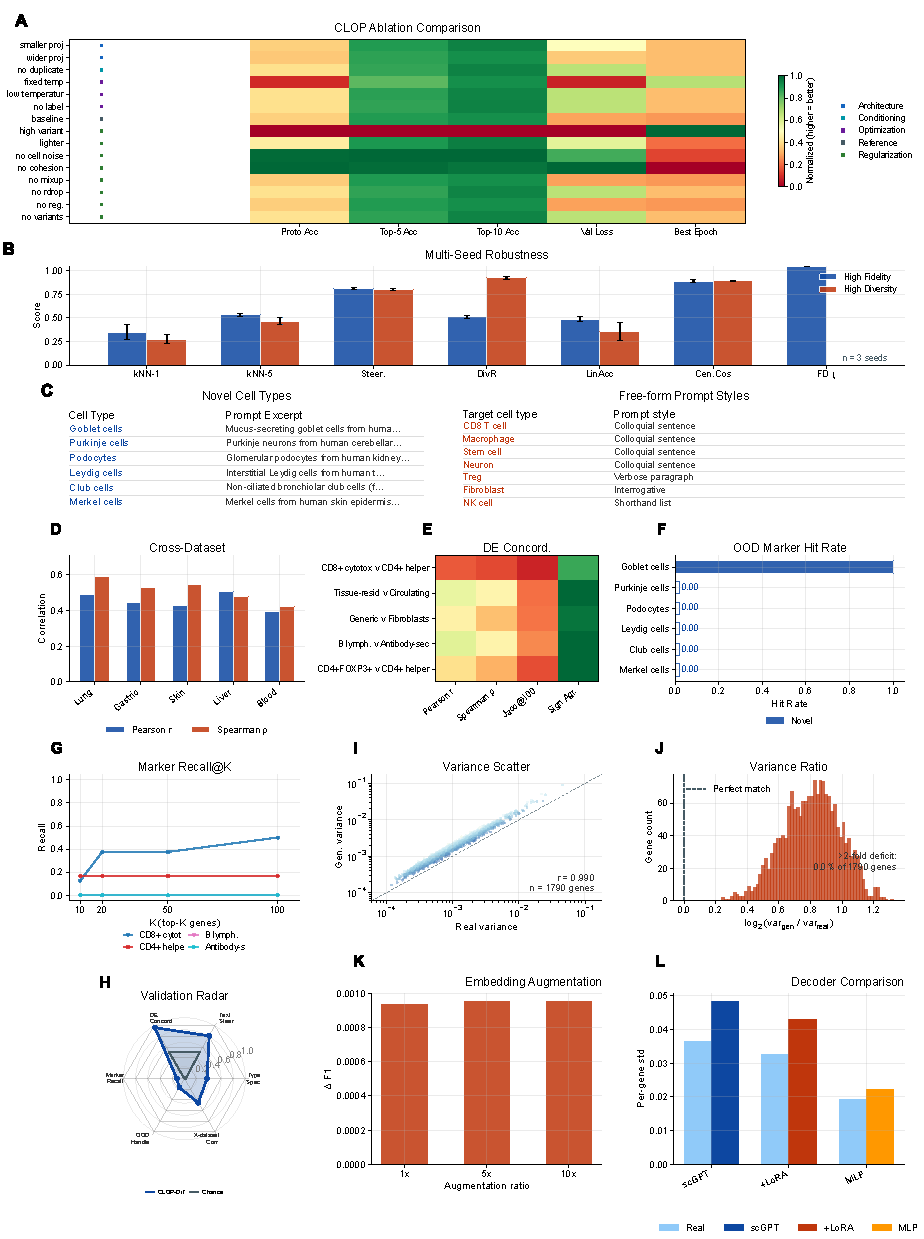
\includegraphics[width=0.88\textwidth]{Figure_A1_supplementary_validation.pdf}
\caption{\textbf{Supplementary validation, ablation, and expression fidelity.}
\textbf{A--C}~Robustness and ablation: CLOP ablations, multi-seed robustness, and the OOD prompt showcase.
\textbf{D--H}~Downstream validation: cross-dataset expression correlation, differential-expression concordance, OOD marker hits, marker recall@$K$, and the six-axis validation radar.
\textbf{I--L}~Expression fidelity and decoder analysis: per-gene variance, variance-ratio deficit, embedding-level augmentation $\Delta$F1, and frozen/LoRA/MLP decoder comparison.\label{fig:ablation-heatmap}\label{fig:multi-seed}\label{fig:ood-showcase}\label{fig:cross-dataset}\label{fig:expanded-de}\label{fig:ood-robustness}\label{fig:marker-completeness}\label{fig:validation-summary}\label{fig:variance-deepdive}\label{fig:embedding-augmentation}\label{fig:decoder-ablation}}
\end{figure}

\begin{figure}[!htbp]
\centering
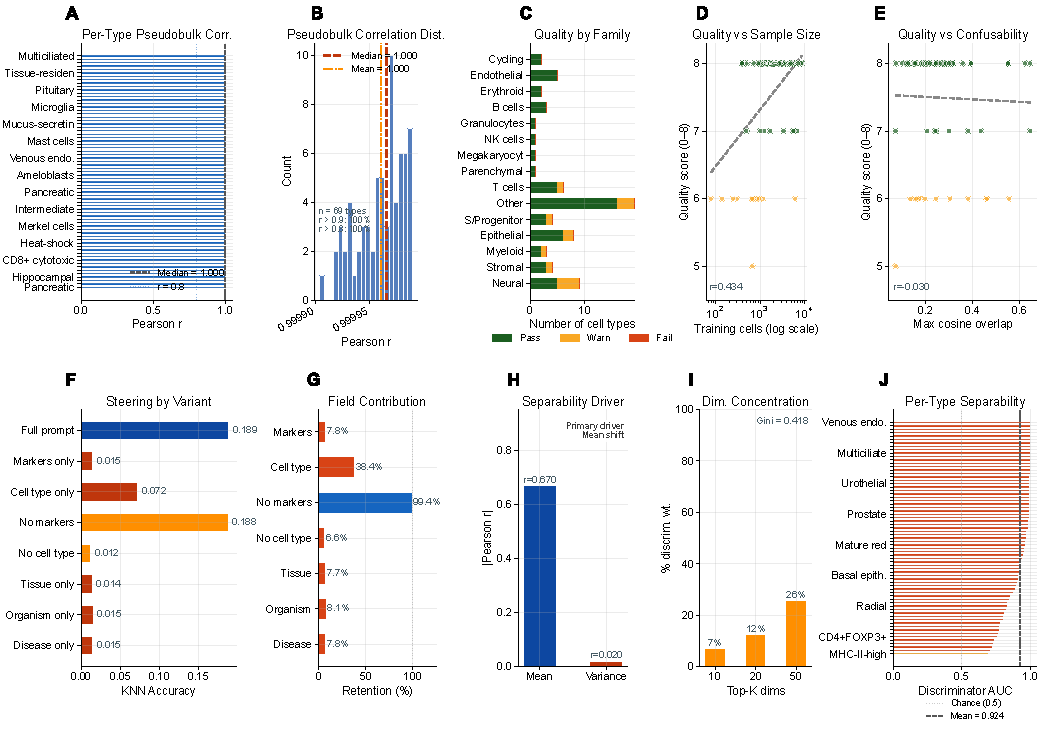
\includegraphics[width=\textwidth]{Figure_A2_expression_diagnostics.pdf}
\caption{\textbf{Expression-level validation and diagnostic analyses.}
\textbf{A, B}~Per-cell-type pseudobulk correlation between real and generated mean-expression profiles ($n = 69$ types): (A)~sorted Pearson~$r$ per type and (B)~distribution of correlations with median and mean indicators.
\textbf{C--E}~Failure-mode analysis: (C)~quality-tier distribution (pass/warn/fail) stratified by biological family, (D)~quality score versus training sample size (Pearson~$r = 0.43$), and (E)~quality score versus embedding confusability (Pearson~$r = -0.03$), indicating that generation quality scales with data abundance but is robust to inter-type similarity.
\textbf{F, G}~Prompt-field ablation: (F)~per-variant KNN accuracy showing that the cell-type field dominates steering effectiveness, and (G)~retention relative to the full prompt (cell type alone retains 38\,\%; removing the cell type drops accuracy to 7\,\%).
\textbf{H--J}~Discriminator feature importance: (H)~separability is primarily mean-driven ($|r| = 0.67$) rather than variance-driven, (I)~discriminative-weight concentration across embedding dimensions (Gini coefficient = 0.42), and (J)~per-type real-versus-generated AUC distribution (mean AUC = 0.92).\label{fig:pseudobulk}\label{fig:failure-analysis}\label{fig:field-ablation}\label{fig:discriminator}}
\end{figure}

\begin{figure}[!htbp]
\centering
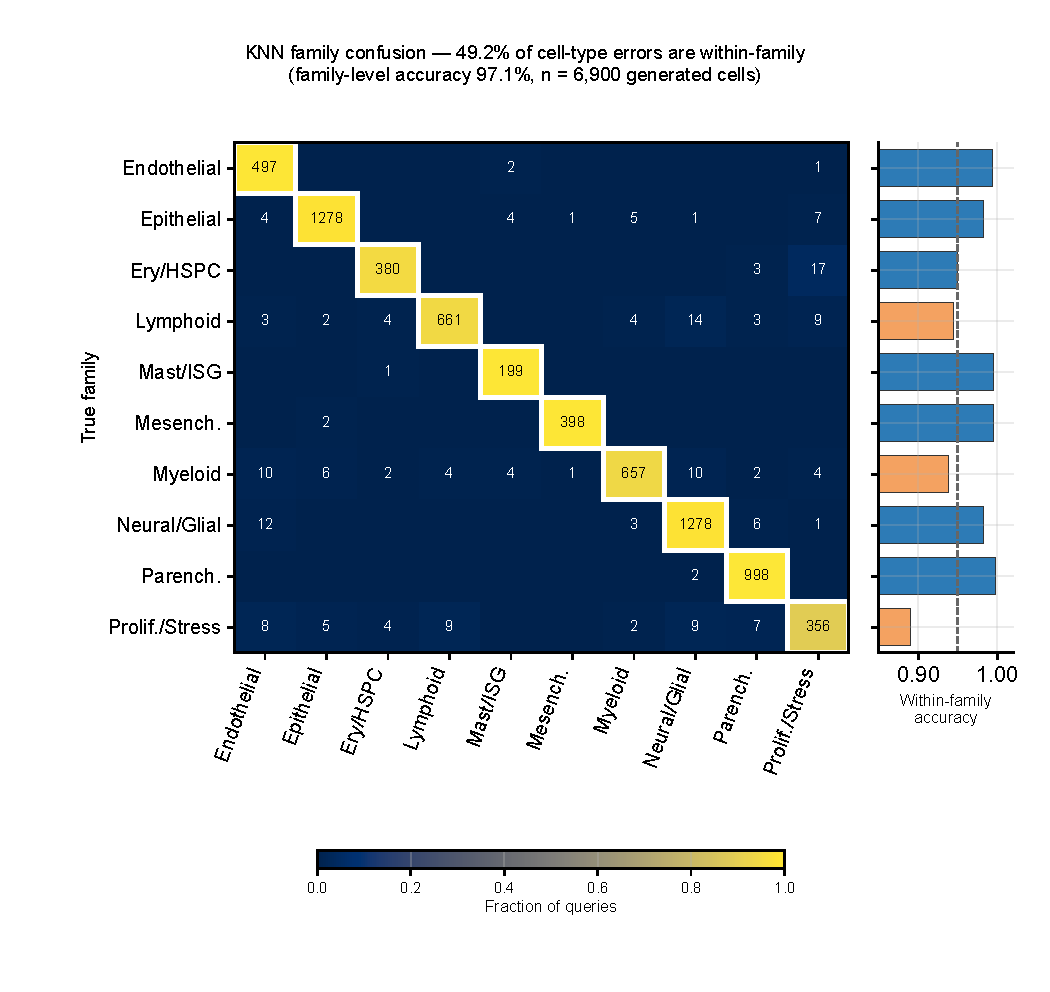
\includegraphics[width=\textwidth]{Figure_A3_knn_family_heatmap.pdf}
\caption{\textbf{KNN error taxonomy across a 10-family biologically-grounded cell-lineage map.} True-family rows against predicted-family columns for every mis-typed cell across the 69 evaluation cell types; diagonal cells (highlighted) report the fraction of errors that remain within the same lineage family. Overall within-family error fraction is 49.2\%, consistent with the claim that approximately half of KNN mis-typings are graceful lineage-adjacent confusions rather than cross-lineage failures. Right-side marginal: per-family within-family-error rate, showing that every family except proliferation/stress/pluripotent maintains within-family accuracy $\geq 0.94$.\label{fig:knn-family-heatmap}}
\end{figure}

\begin{figure}[!htbp]
\centering
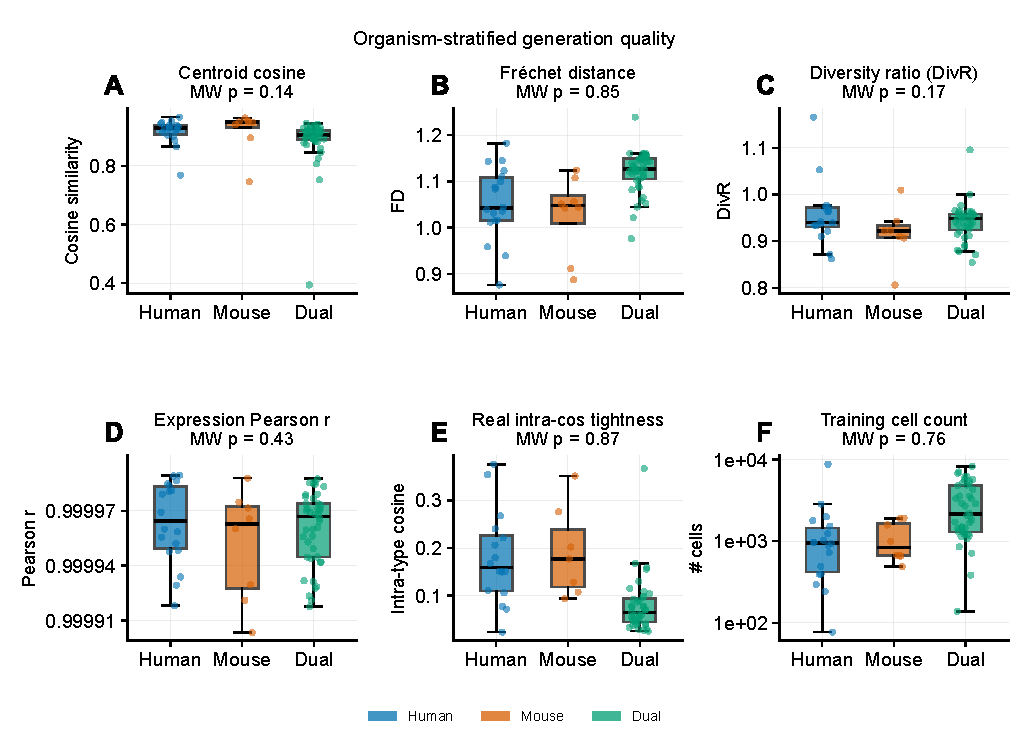
\includegraphics[width=0.98\textwidth]{Figure_A4_organism_stratified.pdf}
\caption{\textbf{Organism-stratified per-type evaluation.} Box-and-whisker distributions of six headline per-type metrics --- \textbf{A}~centroid cosine, \textbf{B}~Fr\'echet distance, \textbf{C}~diversity ratio, \textbf{D}~expression Pearson $r$, \textbf{E}~real within-type cosine tightness, \textbf{F}~log$_{10}$ training cell count --- partitioned across 18 human-only, 8 mouse-only, and 43 dual-organism cell types. Panel headers report Mann--Whitney $p$-values (human vs.\ mouse): 0.14 / 0.85 / 0.17 / 0.43 / 0.87 / 0.76 respectively, confirming no statistically significant species bias at the type level despite the 59/21 dataset-count imbalance.\label{fig:organism-stratified}}
\end{figure}

\begin{figure}[!htbp]
\centering
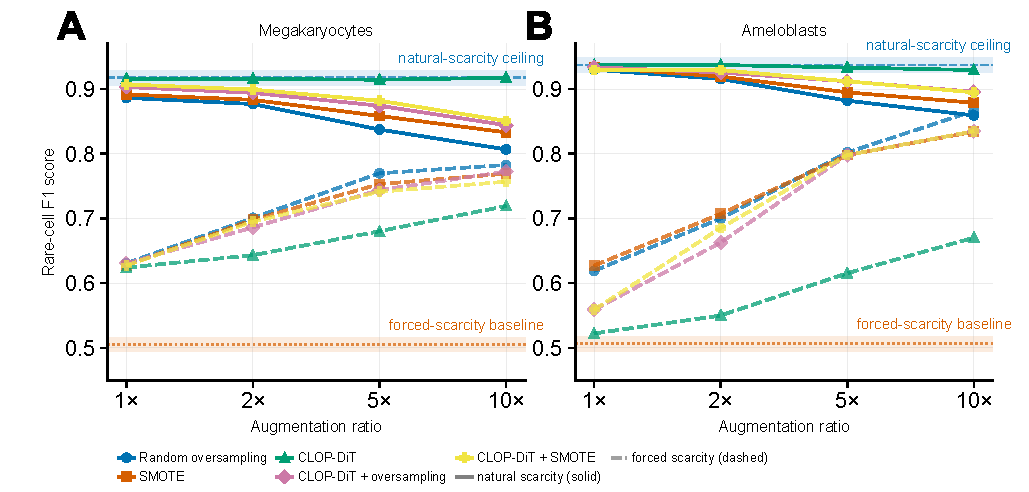
\includegraphics[width=0.98\textwidth]{Figure_A5_forced_scarcity.pdf}
\caption{\textbf{Forced-scarcity rescue: augmentation works when there is real headroom.} Rare-class F1 as a function of augmentation ratio ($1\times$, $2\times$, $5\times$, $10\times$) for two cell types --- \textbf{A}~Megakaryocytes, \textbf{B}~Ameloblasts --- under two scarcity regimes: natural scarcity (solid lines, baseline F1 $\geq 0.92$) and forced scarcity with 30 training cells per class (dashed lines, baseline F1 $\approx 0.50$). Five strategies compared: random oversampling, SMOTE, CLOP-DiT-only, CLOP-DiT + oversampling, CLOP-DiT + SMOTE. Augmentation is flat or mildly negative under natural scarcity (ceiling-driven null) but recovers F1 by 0.2--0.35 under forced scarcity. The natural-scarcity null is therefore a ceiling artefact rather than a principled augmentation failure.\label{fig:forced-scarcity}}
\end{figure}

\FloatBarrier  % Force all appendix floats to appear before the reference list
\clearpage

\begin{adjustwidth}{-\extralength}{0cm}
%} % If the paper is ``preprints'', please uncomment this parenthesis.
%\printendnotes[custom] % Un-comment to print a list of endnotes

% Thebibliography already provides the references heading; avoid a duplicate
% standalone title block here.

% Please provide the correct journal abbreviation (e.g. according to the “List of Title Word Abbreviations” http://www.issn.org/services/online-services/access-to-the-ltwa/).
% Citations and References in Supplementary files are permitted provided that they also appear in the reference list here. 

%=====================================
% References, variant A: external bibliography
%=====================================
%% NOTE: Variant A is not used. All references are inline below.

%=====================================
% References, variant B: internal bibliography
%=====================================

% ACS format — ordered by first citation appearance in the text
\begin{thebibliography}{999}
\setlength{\itemsep}{0pt}\setlength{\parskip}{0pt}\setlength{\parsep}{0pt}

\bibitem{ref-scrnaseq-review}
Svensson,~V.; Vento-Tormo,~R.; Teichmann,~S.A. Exponential scaling of single-cell RNA-seq in the past decade. {\em Nat.\ Protoc.} {\bf 2018}, {\em 13}, 599--604.

\bibitem{ref-10x}
Zheng,~G.X.Y.; Terry,~J.M.; Belgrader,~P.; Ryvkin,~P.; Bent,~Z.W.; Wilson,~R.; Ziraldo,~S.B.; Wheeler,~T.D.; McDermott,~G.P.; Zhu,~J.; et~al. Massively parallel digital transcriptional profiling of single cells. {\em Nat.\ Commun.} {\bf 2017}, {\em 8}, 14049.

\bibitem{ref-scvi}
Lopez,~R.; Regier,~J.; Cole,~M.B.; Jordan,~M.I.; Yosef,~N. Deep generative modeling for single-cell transcriptomics. {\em Nat.\ Methods} {\bf 2018}, {\em 15}, 1053--1058.

\bibitem{ref-scvi-tools}
Gayoso,~A.; Lopez,~R.; Xing,~G.; Boyeau,~P.; Wu,~K.V.; Jayasuriya,~M.; Mehlman,~E.; Lancel,~M.; Regier,~J.; et~al. A Python library for probabilistic analysis of single-cell omics data. {\em Nat.\ Biotechnol.} {\bf 2022}, {\em 40}, 163--166.

\bibitem{ref-scgen}
Lotfollahi,~M.; Wolf,~F.A.; Theis,~F.J. scGen predicts single-cell perturbation responses. {\em Nat.\ Methods} {\bf 2019}, {\em 16}, 715--721.

\bibitem{ref-scdiff}
Ding,~J.; Regev,~A. Deep generative model embedding of single-cell RNA-Seq profiles on hyperspheres and hyperbolic spaces. {\em Nat.\ Commun.} {\bf 2021}, {\em 12}, 2554.

\bibitem{ref-geneformer}
Theodoris,~C.V.; Xiao,~L.; Chopra,~A.; Chaffin,~M.D.; Al Sayed,~Z.R.; Hill,~M.C.; Mantineo,~H.; Brydon,~E.M.; Zeng,~Z.; Liu,~X.S.; et~al. Transfer learning enables predictions in network biology. {\em Nature} {\bf 2023}, {\em 618}, 616--624.

\bibitem{ref-scbert}
Yang,~F.; Wang,~W.; Wang,~F.; Fang,~Y.; Tang,~D.; Huang,~J.; Lu,~H.; Yao,~J. scBERT as a large-scale pretrained deep language model for cell type annotation of single-cell RNA-seq data. {\em Nat.\ Mach.\ Intell.} {\bf 2022}, {\em 4}, 852--861.

\bibitem{ref-scfoundation}
Hao,~M.; Gong,~J.; Zeng,~X.; Liu,~C.; Guo,~Y.; Cheng,~X.; Wang,~T.; Ma,~J.; Zhang,~X.; Song,~L. Large-scale foundation model on single-cell transcriptomics. {\em Nat.\ Methods} {\bf 2024}, {\em 21}, 1481--1491.

\bibitem{ref-cellplm}
Wen,~H.; Tang,~W.; Dai,~X.; Ding,~J.; Jin,~W.; Xie,~Y.; Tang,~J. CellPLM: Pre-training of cell language model beyond single cells. Presented at the 12th International Conference on Learning Representations (ICLR 2024), Poster, Vienna, Austria, 7--11 May 2024. Available online: \url{https://openreview.net/forum?id=BKXvPDekud} (accessed on 29 March 2026).

\bibitem{ref-uce}
Rosen,~Y.; Roohani,~Y.H.; Agrawal,~A.; Leskovec,~J. Universal cell embeddings: A foundation model for cell biology. Preprint at bioRxiv \url{https://doi.org/10.1101/2023.11.28.568918} (2023).

\bibitem{ref-cell2sentence}
Levine,~D.; Rizvi,~S.A.; L\'{e}vy,~S.; Pallikkavaliyaveetil,~N.; Zhang,~D.; Chen,~X.; Ghadermarzi,~S.; Wu,~R.; Zheng,~Z.; Vrkic,~I.; et~al. Cell2Sentence: Teaching Large Language Models the Language of Biology. Presented at the 41st International Conference on Machine Learning (ICML 2024), Poster, Vienna, Austria, 21--27 July 2024. Available online: \url{https://openreview.net/forum?id=EWt5wsEdvc} (accessed on 29 March 2026).

\bibitem{ref-genept}
Chen,~Y.; Zou,~J. Simple and effective embedding model for single-cell biology built from ChatGPT. {\em Nat.\ Biomed.\ Eng.} {\bf 2025}, {\em 9}, 483--493.

\bibitem{ref-clip}
Radford,~A.; Kim,~J.W.; Hallacy,~C.; Ramesh,~A.; Goh,~G.; Agarwal,~S.; Sastry,~G.; Askell,~A.; Mishkin,~P.; Clark,~J.; et~al. Learning transferable visual models from natural language supervision. In Proceedings of the 38th International Conference on Machine Learning (ICML), Virtual, 18--24 July 2021; pp.\ 8748--8763.

\bibitem{ref-siglip}
Zhai,~X.; Mustafa,~B.; Kolesnikov,~A.; Beyer,~L. Sigmoid loss for language image pre-training. In Proceedings of the IEEE/CVF International Conference on Computer Vision (ICCV), Paris, France, 2--6 October 2023; pp.\ 11975--11986.

\bibitem{ref-dit}
Peebles,~W.; Xie,~S. Scalable diffusion models with transformers. In Proceedings of the IEEE/CVF International Conference on Computer Vision (ICCV), Paris, France, 2--6 October 2023; pp.\ 4195--4205.

\bibitem{ref-flow-matching}
Lipman,~Y.; Chen,~R.T.Q.; Ben-Hamu,~H.; Nickel,~M. Flow matching for generative modeling. In Proceedings of the 11th International Conference on Learning Representations (ICLR), Kigali, Rwanda, 1--5 May 2023.

\bibitem{ref-albergo-flow}
Albergo,~M.S.; Vanden-Eijnden,~E. Building normalizing flows with stochastic interpolants. In Proceedings of the 11th International Conference on Learning Representations (ICLR), Kigali, Rwanda, 1--5 May 2023.

\bibitem{ref-rectified-flow}
Liu,~X.; Gong,~C.; Liu,~Q. Flow straight and fast: Learning to generate and transfer data with rectified flow. In Proceedings of the 11th International Conference on Learning Representations (ICLR), Kigali, Rwanda, 1--5 May 2023.

\bibitem{ref-seurat}
Stuart,~T.; Butler,~A.; Hoffman,~P.; Hafemeister,~C.; Papalexi,~E.; Mauck,~W.M.; Hao,~Y.; Stoeckius,~M.; Smibert,~P.; Satija,~R. Comprehensive integration of single-cell data. {\em Cell} {\bf 2019}, {\em 177}, 1888--1902.

\bibitem{ref-hvg}
Brennecke,~P.; Anders,~S.; Kim,~J.K.; Kolodziejczyk,~A.A.; Zhang,~X.; Proserpio,~V.; Baying,~B.; Benes,~V.; Teichmann,~S.A.; Marioni,~J.C.; Heisler,~M.G. Accounting for technical noise in single-cell RNA-seq experiments. {\em Nat.\ Methods} {\bf 2013}, {\em 10}, 1093--1095.

\bibitem{ref-wilcoxon}
Wilcoxon,~F. Individual comparisons by ranking methods. {\em Biom.\ Bull.} {\bf 1945}, {\em 1}, 80--83.

\bibitem{ref-panglao}
Franz\'{e}n,~O.; Gan,~L.M.; Bj\"{o}rkegren,~J.L.M. PanglaoDB: A web server for exploration of mouse and human single-cell RNA sequencing data. {\em Database} {\bf 2019}, {\em 2019}, baz046.

\bibitem{ref-cellmarker}
Hu,~C.; Li,~T.; Xu,~Y.; Zhang,~X.; Li,~F.; Bai,~J.; Chen,~J.; Jiang,~W.; Yang,~K.; Ou,~Q.; et~al. CellMarker~2.0: An updated database of manually curated cell markers in human/mouse and web tools based on scRNA-seq data. {\em Nucleic Acids Res.} {\bf 2023}, {\em 51}, D870--D876.

\bibitem{ref-leiden}
Traag,~V.A.; Waltman,~L.; van~Eck,~N.J. From Louvain to Leiden: Guaranteeing well-connected communities. {\em Sci. Rep.} {\bf 2019}, {\em 9}, 5233.

\bibitem{ref-tabula-muris}
Tabula Muris Consortium. Single-cell transcriptomics of 20 mouse organs creates a Tabula Muris. {\em Nature} {\bf 2018}, {\em 562}, 367--372.

\bibitem{ref-batchnorm}
Ioffe,~S.; Szegedy,~C. Batch normalization: Accelerating deep network training by reducing internal covariate shift. In Proceedings of the 32nd International Conference on Machine Learning (ICML), Lille, France, 6--11 July 2015; pp.\ 448--456.

\bibitem{ref-gelu}
Hendrycks,~D.; Gimpel,~K. Gaussian error linear units (GELUs). {\em arXiv} {\bf 2016}, 1606.08415.

\bibitem{ref-dropout}
Srivastava,~N.; Hinton,~G.; Krizhevsky,~A.; Sutskever,~I.; Salakhutdinov,~R. Dropout: A simple way to prevent neural networks from overfitting. {\em J.\ Mach.\ Learn.\ Res.} {\bf 2014}, {\em 15}, 1929--1958.

\bibitem{ref-adamw}
Loshchilov,~I.; Hutter,~F. Decoupled weight decay regularization. In Proceedings of the 7th International Conference on Learning Representations (ICLR), New Orleans, LA, USA, 6--9 May 2019.

\bibitem{ref-cosine-schedule}
Loshchilov,~I.; Hutter,~F. SGDR: Stochastic gradient descent with warm restarts. In Proceedings of the 5th International Conference on Learning Representations (ICLR), Toulon, France, 24--26 April 2017.

\bibitem{ref-ot-cfm}
Tong,~A.; Malkin,~N.; Huguet,~G.; Zhang,~Y.; Rector-Brooks,~J.; Fatras,~K.; Wolf,~G.; Bengio,~Y. Improving and generalizing flow-based generative models with minibatch optimal transport. {\em Trans.\ Mach.\ Learn.\ Res.} {\bf 2024}.

\bibitem{ref-sd3}
Esser,~P.; Kulal,~S.; Blattmann,~A.; Entezari,~R.; M\"{u}ller,~J.; Saini,~H.; Levi,~Y.; Lorenz,~D.; Sauer,~A.; Boesel,~F.; et~al. Scaling rectified flow transformers for high-resolution image synthesis. Preprint at arXiv \url{https://doi.org/10.48550/arXiv.2403.03206} (2024).

\bibitem{ref-cfg}
Ho,~J.; Salimans,~T. Classifier-free diffusion guidance. In Proceedings of the NeurIPS 2021 Workshop on Deep Generative Models and Downstream Applications, Virtual, 13 December 2021.

\bibitem{ref-ema}
Polyak,~B.T.; Juditsky,~A.B. Acceleration of stochastic approximation by averaging. {\em SIAM J.\ Control Optim.} {\bf 1992}, {\em 30}, 838--855.

\bibitem{ref-ari}
Hubert,~L.; Arabie,~P. Comparing partitions. {\em J.\ Classif.} {\bf 1985}, {\em 2}, 193--218.

\bibitem{ref-nmi}
Strehl,~A.; Ghosh,~J. Cluster ensembles---A knowledge reuse framework for combining multiple partitions. {\em J.\ Mach.\ Learn.\ Res.} {\bf 2002}, {\em 3}, 583--617.

\bibitem{ref-fid}
Heusel,~M.; Ramsauer,~H.; Unterthiner,~T.; Nessler,~B.; Hochreiter,~S. GANs trained by a two time-scale update rule converge to a local Nash equilibrium. {\em Adv.\ Neural Inf.\ Process.\ Syst.} {\bf 2017}, {\em 30}, 6626--6637.

\bibitem{ref-umap}
McInnes,~L.; Healy,~J.; Melville,~J. UMAP: Uniform manifold approximation and projection for dimension reduction. {\em arXiv} {\bf 2018}, 1802.03426.

\bibitem{ref-scanpy}
Wolf,~F.A.; Angerer,~P.; Theis,~F.J. SCANPY: Large-scale single-cell gene expression data analysis. {\em Genome Biol.} {\bf 2018}, {\em 19}, 15.

\bibitem{ref-integration-benchmark}
Luecken,~M.D.; Buttner,~M.; Chaichoompu,~K.; Danese,~A.; Interlandi,~M.; Mueller,~M.F.; Strobl,~D.C.; Zappia,~L.; Dugas,~M.; Colome-Tatche,~M.; Theis,~F.J. Benchmarking atlas-level data integration in single-cell genomics. {\em Nat.\ Methods} {\bf 2022}, {\em 19}, 41--50.

\bibitem{ref-cellwhisperer}
Schaefer,~M.; Peneder,~P.; Malzl,~D.; Lombardo,~S.D.; Peycheva,~M.; Burton,~J.; Hakobyan,~A.; Sharma,~V.; Krausgruber,~T.; Sin,~C.; et~al. Multimodal learning enables chat-based exploration of single-cell data. {\em Nat.\ Biotechnol.} {\bf 2025}. Advance online publication. \url{https://doi.org/10.1038/s41587-025-02857-9}.

\bibitem{ref-scdesign3}
Song,~D.; Wang,~Q.; Yan,~G.; Liu,~T.; Sun,~T.; Li,~J.J. scDesign3 generates realistic in silico data for multimodal single-cell and spatial omics. {\em Nat.\ Biotechnol.} {\bf 2024}, {\em 42}, 247--252.

\bibitem{ref-scgpt}
Cui,~H.; Wang,~C.; Maan,~H.; Pang,~K.; Luo,~F.; Duan,~N.; Wang,~B. scGPT: Toward building a foundation model for single-cell multi-omics using generative AI. {\em Nat.\ Methods} {\bf 2024}, {\em 21}, 1470--1480.

\bibitem{ref-clop-dit}
Fu,~Z. CLOP-DiT: Structured-Metadata-Conditioned Single-Cell Latent Generation via Contrastive Language-Omics Pretraining and Diffusion Transformers. {\em GitHub repository} {\bf 2026}. Available online: \url{https://github.com/PeterPonyu/CLOP-DiT} (accessed on 29 March 2026).

\end{thebibliography}

% If authors have biography, please use the format below
%\section*{Short Biography of Authors}
%\bio
%{\raisebox{-0.35cm}{\includegraphics[width=3.5cm,height=5.3cm,clip,keepaspectratio]{Definitions/author1.pdf}}}
%{\textbf{Firstname Lastname} Biography of first author}
%
%\bio
%{\raisebox{-0.35cm}{\includegraphics[width=3.5cm,height=5.3cm,clip,keepaspectratio]{Definitions/author2.pdf}}}
%{\textbf{Firstname Lastname} Biography of second author}

% For the MDPI journals use author-date citation, please follow the formatting guidelines on http://www.mdpi.com/authors/references
% To cite two works by the same author: \citeauthor{ref-journal-1a} (\citeyear{ref-journal-1a}, \citeyear{ref-journal-1b}). This produces: Whittaker (1967, 1975)
% To cite two works by the same author with specific pages: \citeauthor{ref-journal-3a} (\citeyear{ref-journal-3a}, p. 328; \citeyear{ref-journal-3b}, p.475). This produces: Wong (1999, p. 328; 2000, p. 475)

%%%%%%%%%%%%%%%%%%%%%%%%%%%%%%%%%%%%%%%%%%
%% for journal Sci
%\reviewreports{\\
%Reviewer 1 comments and authors’ response\\
%Reviewer 2 comments and authors’ response\\
%Reviewer 3 comments and authors’ response
%}
%%%%%%%%%%%%%%%%%%%%%%%%%%%%%%%%%%%%%%%%%%
\PublishersNote{}
%\isPreprints{}{% This command is only used for ``preprints''.
\end{adjustwidth}
%} % If the paper is ``preprints'', please uncomment this parenthesis.

\end{document}
